%%%%%%%%%%%%%%%%%%%%%%%%%%%%%%%%%%%%%%%%%

\documentclass[11pt,a4paper,sans]{moderncv} % Font sizes: 10, 11, or 12; paper sizes: a4paper, letterpaper, a5paper, legalpaper, executivepaper or landscape; font families: sans or roman


\moderncvstyle{casual} % CV theme - options include: 'casual' (default), 'classic', 'oldstyle' and 'banking'
\moderncvcolor{green} % CV color - options include: 'blue' (default), 'orange', 'green', 'red', 'purple', 'grey' and 'black'

\usepackage{xeCJK}\setCJKmainfont{等线}\usepackage{fontspec}\setmainfont{Arial}

\usepackage{lipsum} % Used for inserting dummy 'Lorem ipsum' text into the template
\usepackage{multicol}


\usepackage[scale=0.75]{geometry} % Reduce document margins
%\setlength{\hintscolumnwidth}{3cm} % Uncomment to change the width of the dates column
%\setlength{\makecvtitlenamewidth}{10cm} % For the 'classic' style, uncomment to adjust the width of the space allocated to your name	

%----------------------------------------------------------------------------------------
%	NAME AND CONTACT INFORMATION SECTION
%----------------------------------------------------------------------------------------

\firstname{} % Your first name
\familyname{窦飞鸿} % Your last name
% All information in this block is optional, comment out any lines you don't need
\title{}
%\address{R.N. 165 Boys Hostel 'D', Vidyanagari }{Baramati, MH 413133}
\mobile{(+0513) 15161132813}
\email{315765038@qq.com}
\photo[90pt][0.5pt]{2} % The first bracket is the picture height, the second is the thickness of the frame around the picture (0pt for no frame)
\quote{}

%----------------------------------------------------------------------------------------

\begin{document}
\thispagestyle{empty}

	\makecvtitle % Print the CV title
	
\section{个人信息}
\cvitem{生日}{1996-09-04}
\cvitem{家庭地址}{南京市浦口区象山路5号}
%\cvitem{Languages}{Marathi,Hindi,English}
\cvitem{手机号码}{(+0513) 15161132813}
\cvitem{Email}{315765038@qq.com}
%\cvitem{Social} 
%{\includegraphics[width=0.6cm,height=0.4cm]{facebook}http://www.facebook.com/ermaheshgaikwad}
%\hspace{0.9cm}Network \hspace{0.08cm}
%\includegraphics[width=0.6cm,height=0.4cm]{linkedin}%https://www.linkedin.com/in/maheshgg

%----------------------------------------------------------------------------------------
%	EDUCATION SECTION
%----------------------------------------------------------------------------------------
\section{教育背景}
\cventry{2014.09-至今}{河海大学}{本科在读}{}{}{计算机科学与技术} 
\cventry{2016.09-至今}{河海大学“体育信息实验室”成员}{}{}{\textit{}}{}  % Arguments not required can be left empty
\cventry{2016.09-至今}{河海大学“卓越计划”成员}{}{}{\textit{}}{ }
%\cventry{2007--2008}{Xth Board}{Yashwant Vidyalaya}{Latur}{\textit{Percentage -- 79.53\%}}{Secondary School Certificate}





%------------------------------------------------

\subsection{项目经验}

\cventry{2015.06-2015.08}{上海麦澜运动管理系统}{}{}{}{系统功能:实现对运动场馆的使用管理,并实现用户的预定,消费等功能\\
个人贡献:APP前端页面开发}
\cventry{2015.09-2015.10}{电子信息裁判}{}{}{}{赛事:中华人民共和国第一届全国青年运动会(福建)}
\cventry{2016.11-2017.01}{网咖管理系统}{}{}{}{系统功能:完成前台对网咖机器的日常管理,会员上机,消费等功能\\
个人贡献:数据库的架构与设计,前端交互界面开发
}
\cventry{2015.04-2015.06}{“借阅助手”微信公众平台}{}{}{}{系统功能:通过微信服务号来实现图书馆的图书,会员用户的信息管理,以及相应的借阅功能\\
个人贡献:数据库的架构与设计,前端页面开发
}
\cventry{2017.05-2017.09}{测试工程师(网页开发功能测试),电子信息裁判 }{}{}{}{赛事:中华人民共和国第十三届全国学生运动会(杭州)}
%----------------------------------------------------------------------------------------
%	AWARDS SECTION
%----------------------------------------------------------------------------------------

%----------------------------------------------------------------------------------------
%	COMPUTER SKILLS SECTION
%----------------------------------------------------------------------------------------

\section{技能}

%\subsection{Mechanical Engineering Softwares:}
%\begin{multicols}{3}
%\cvitem {}
%{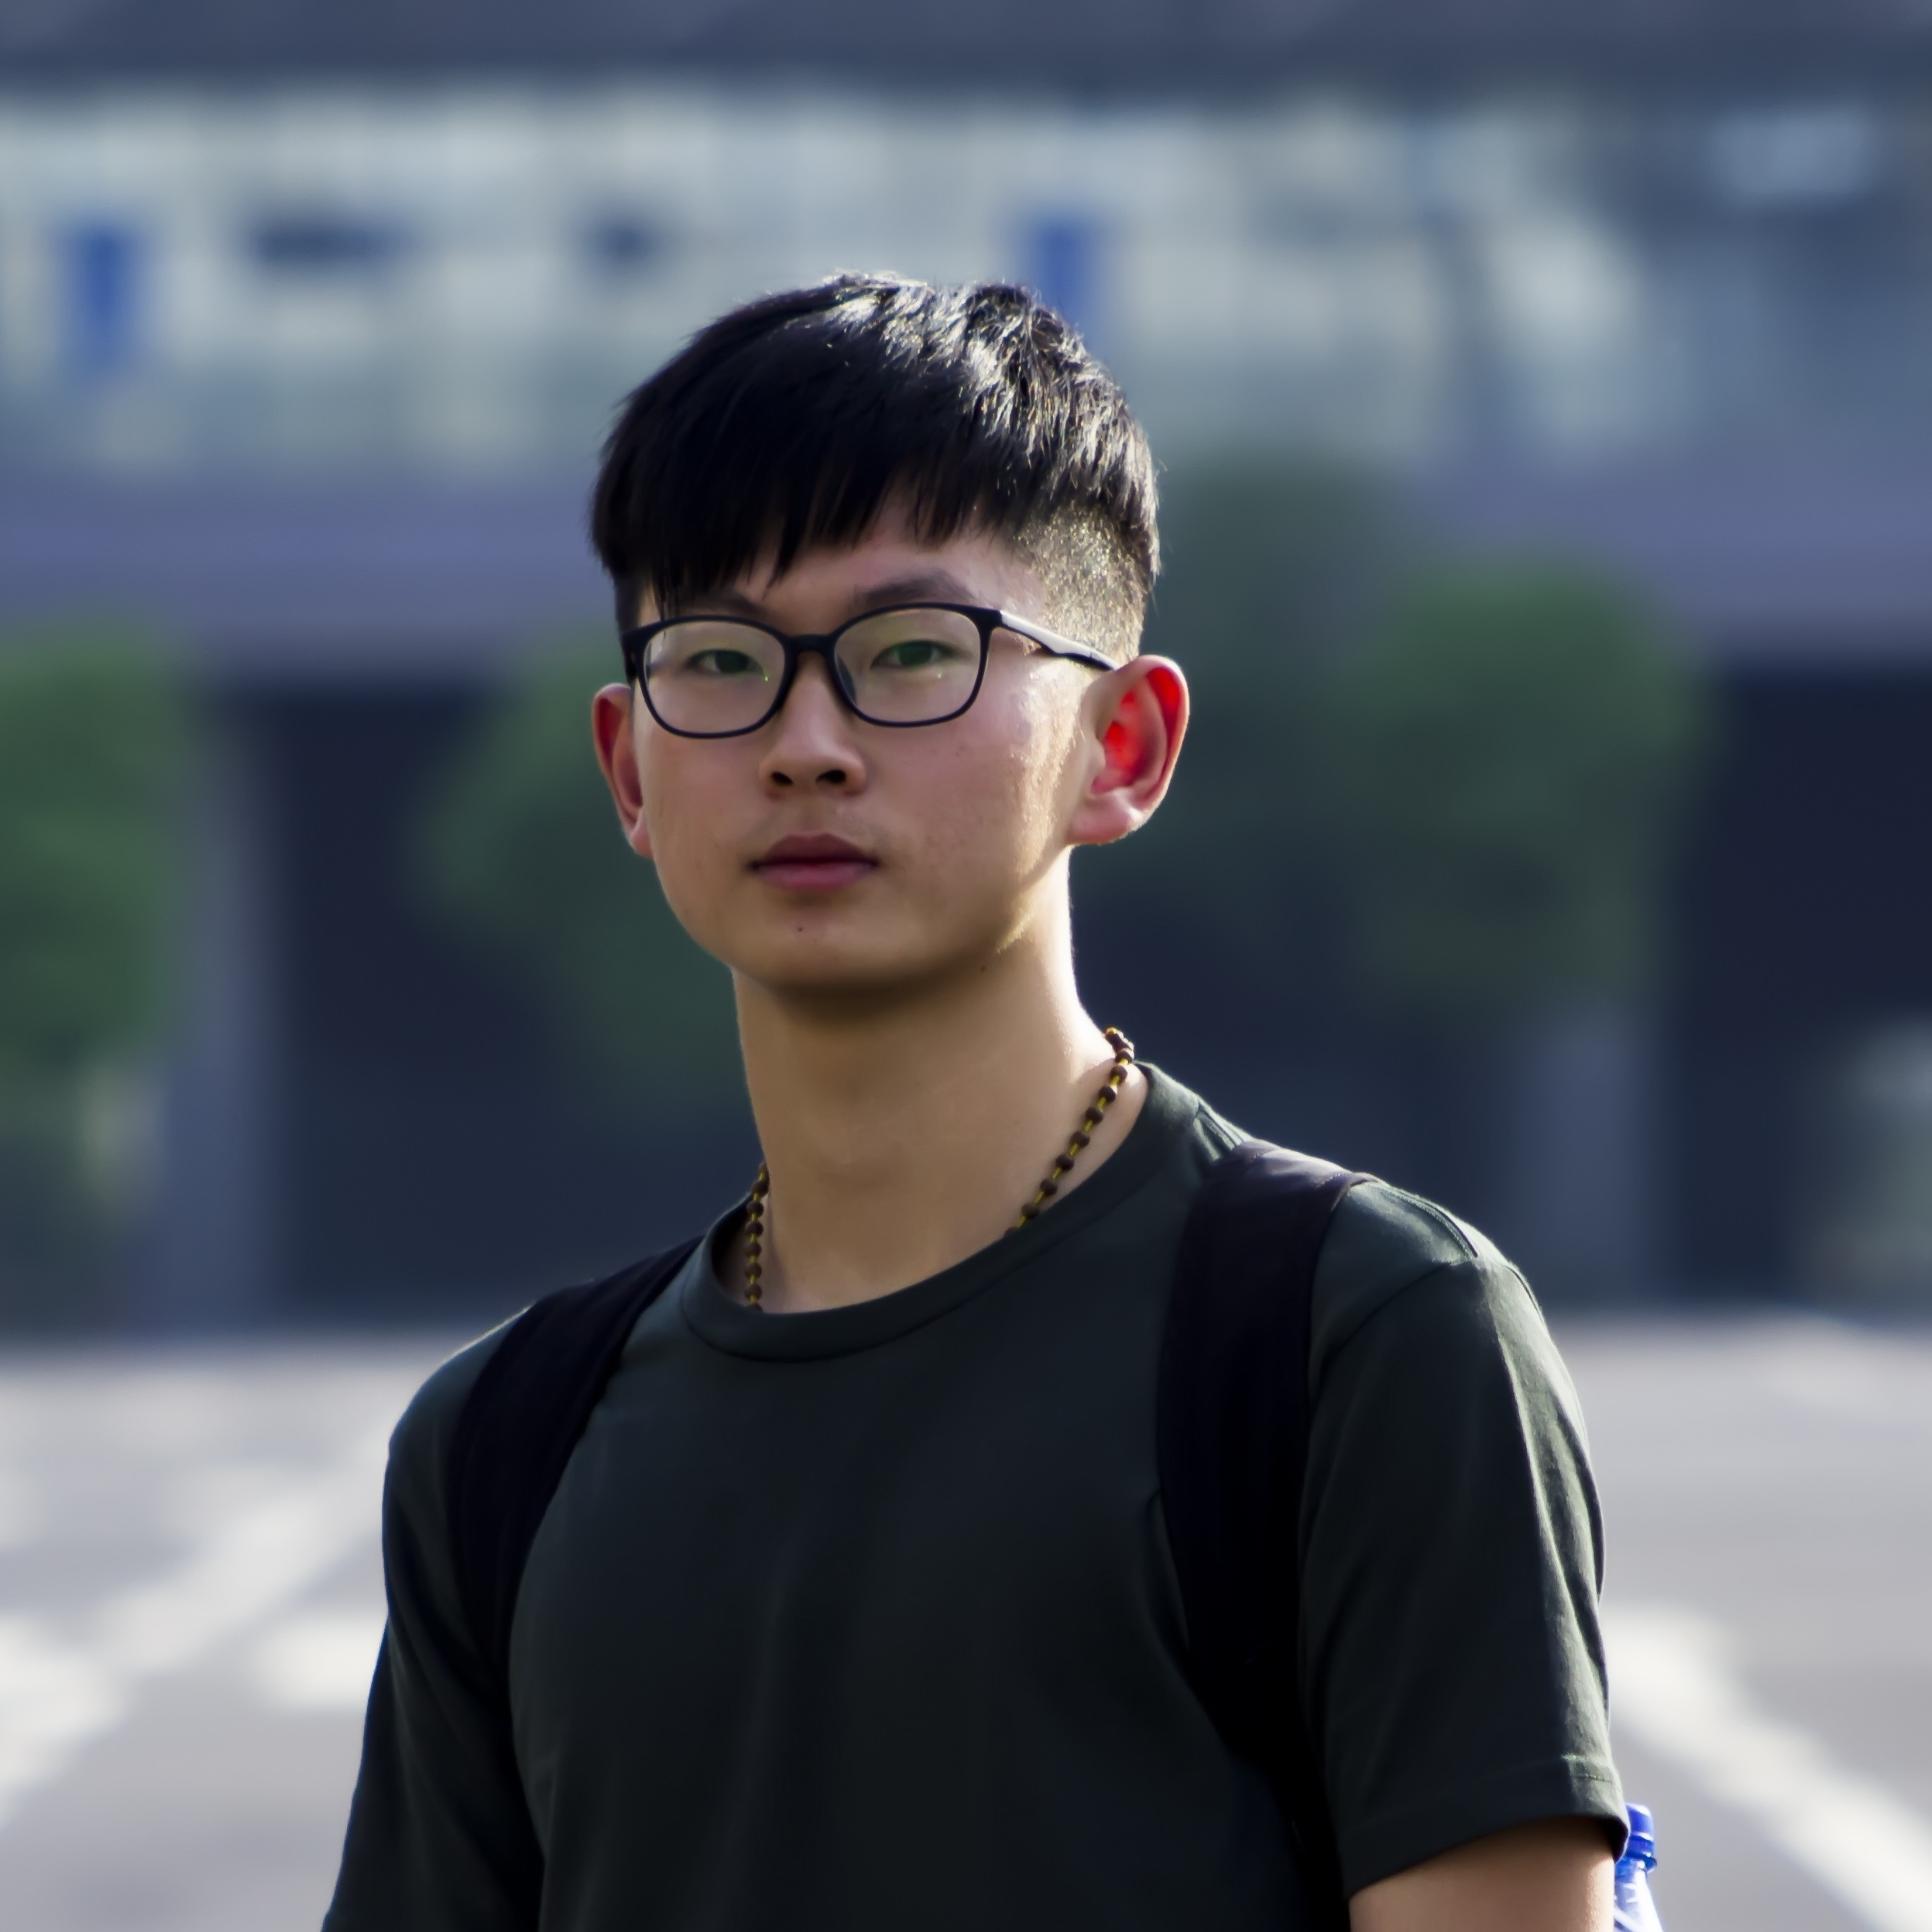
\includegraphics[width=3cm,height=0.7cm]{picture}}
%\cvitem {}{\includegraphics[width=3cm,height=0.7cm]%{picture}}
%\cvitem {}{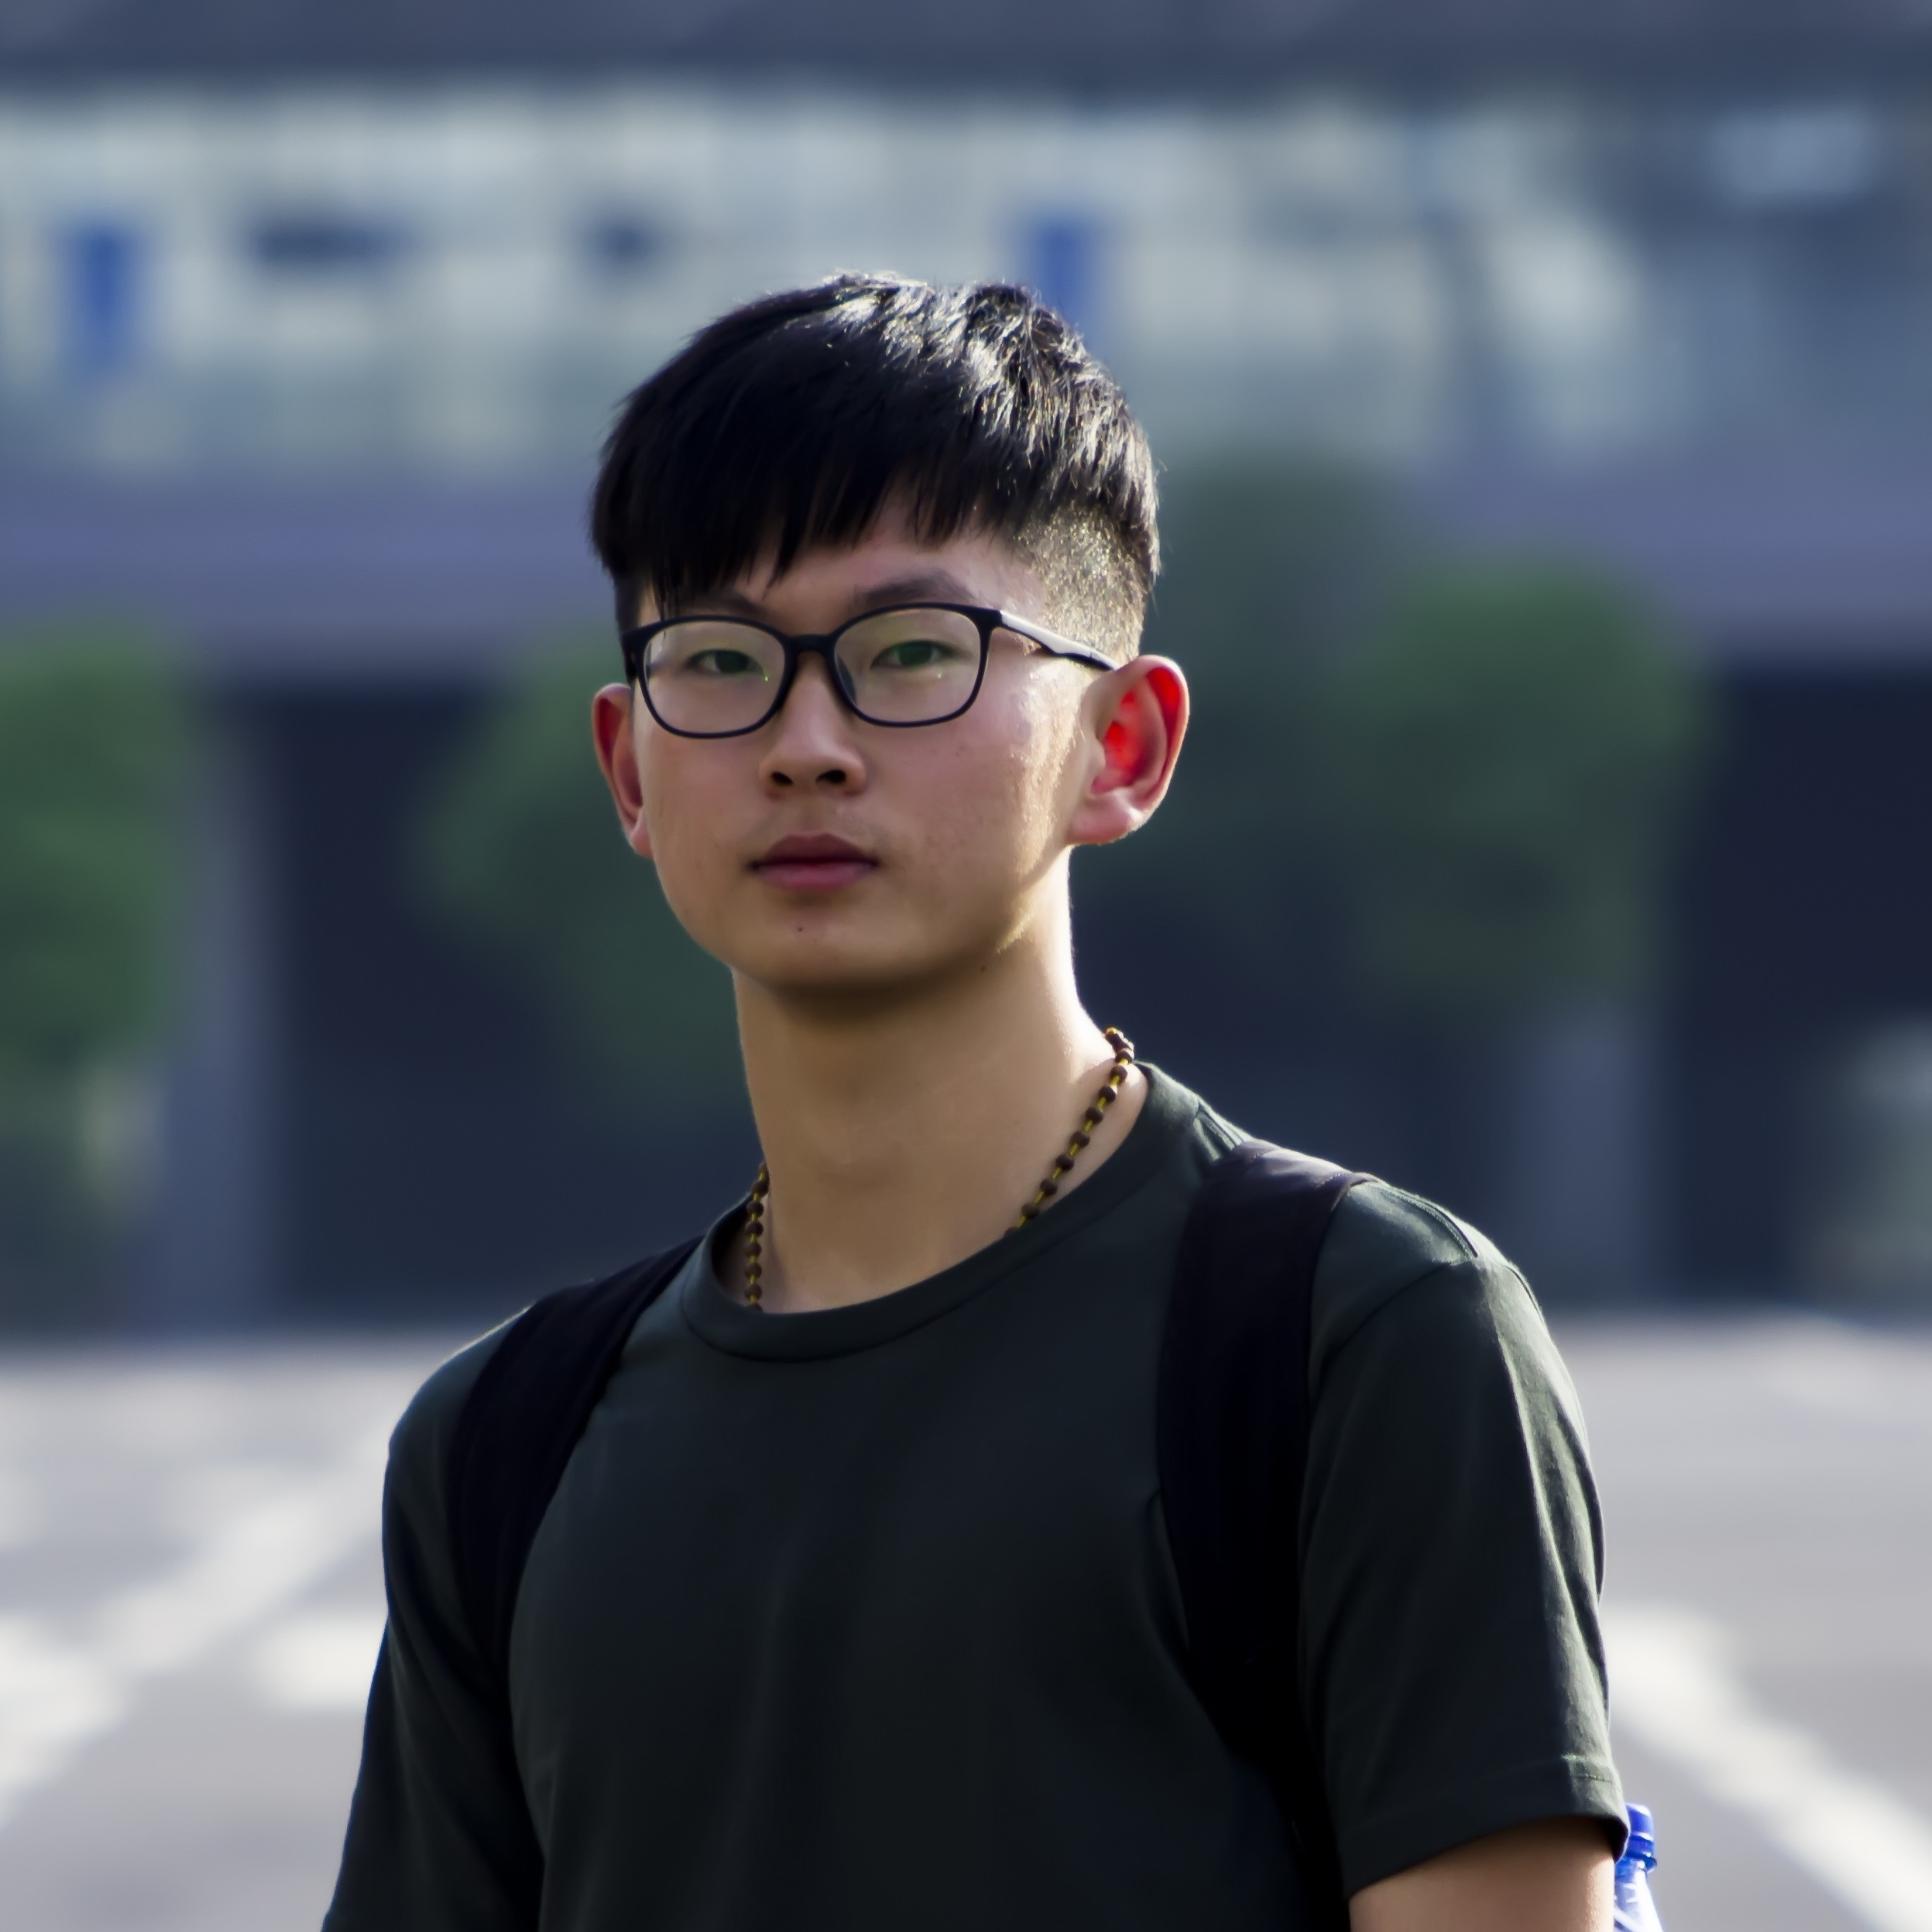
\includegraphics[width=3cm,height=0.7cm]{picture}}
%\end{multicols}
%\begin{multicols}{3}
%\cvitem {}{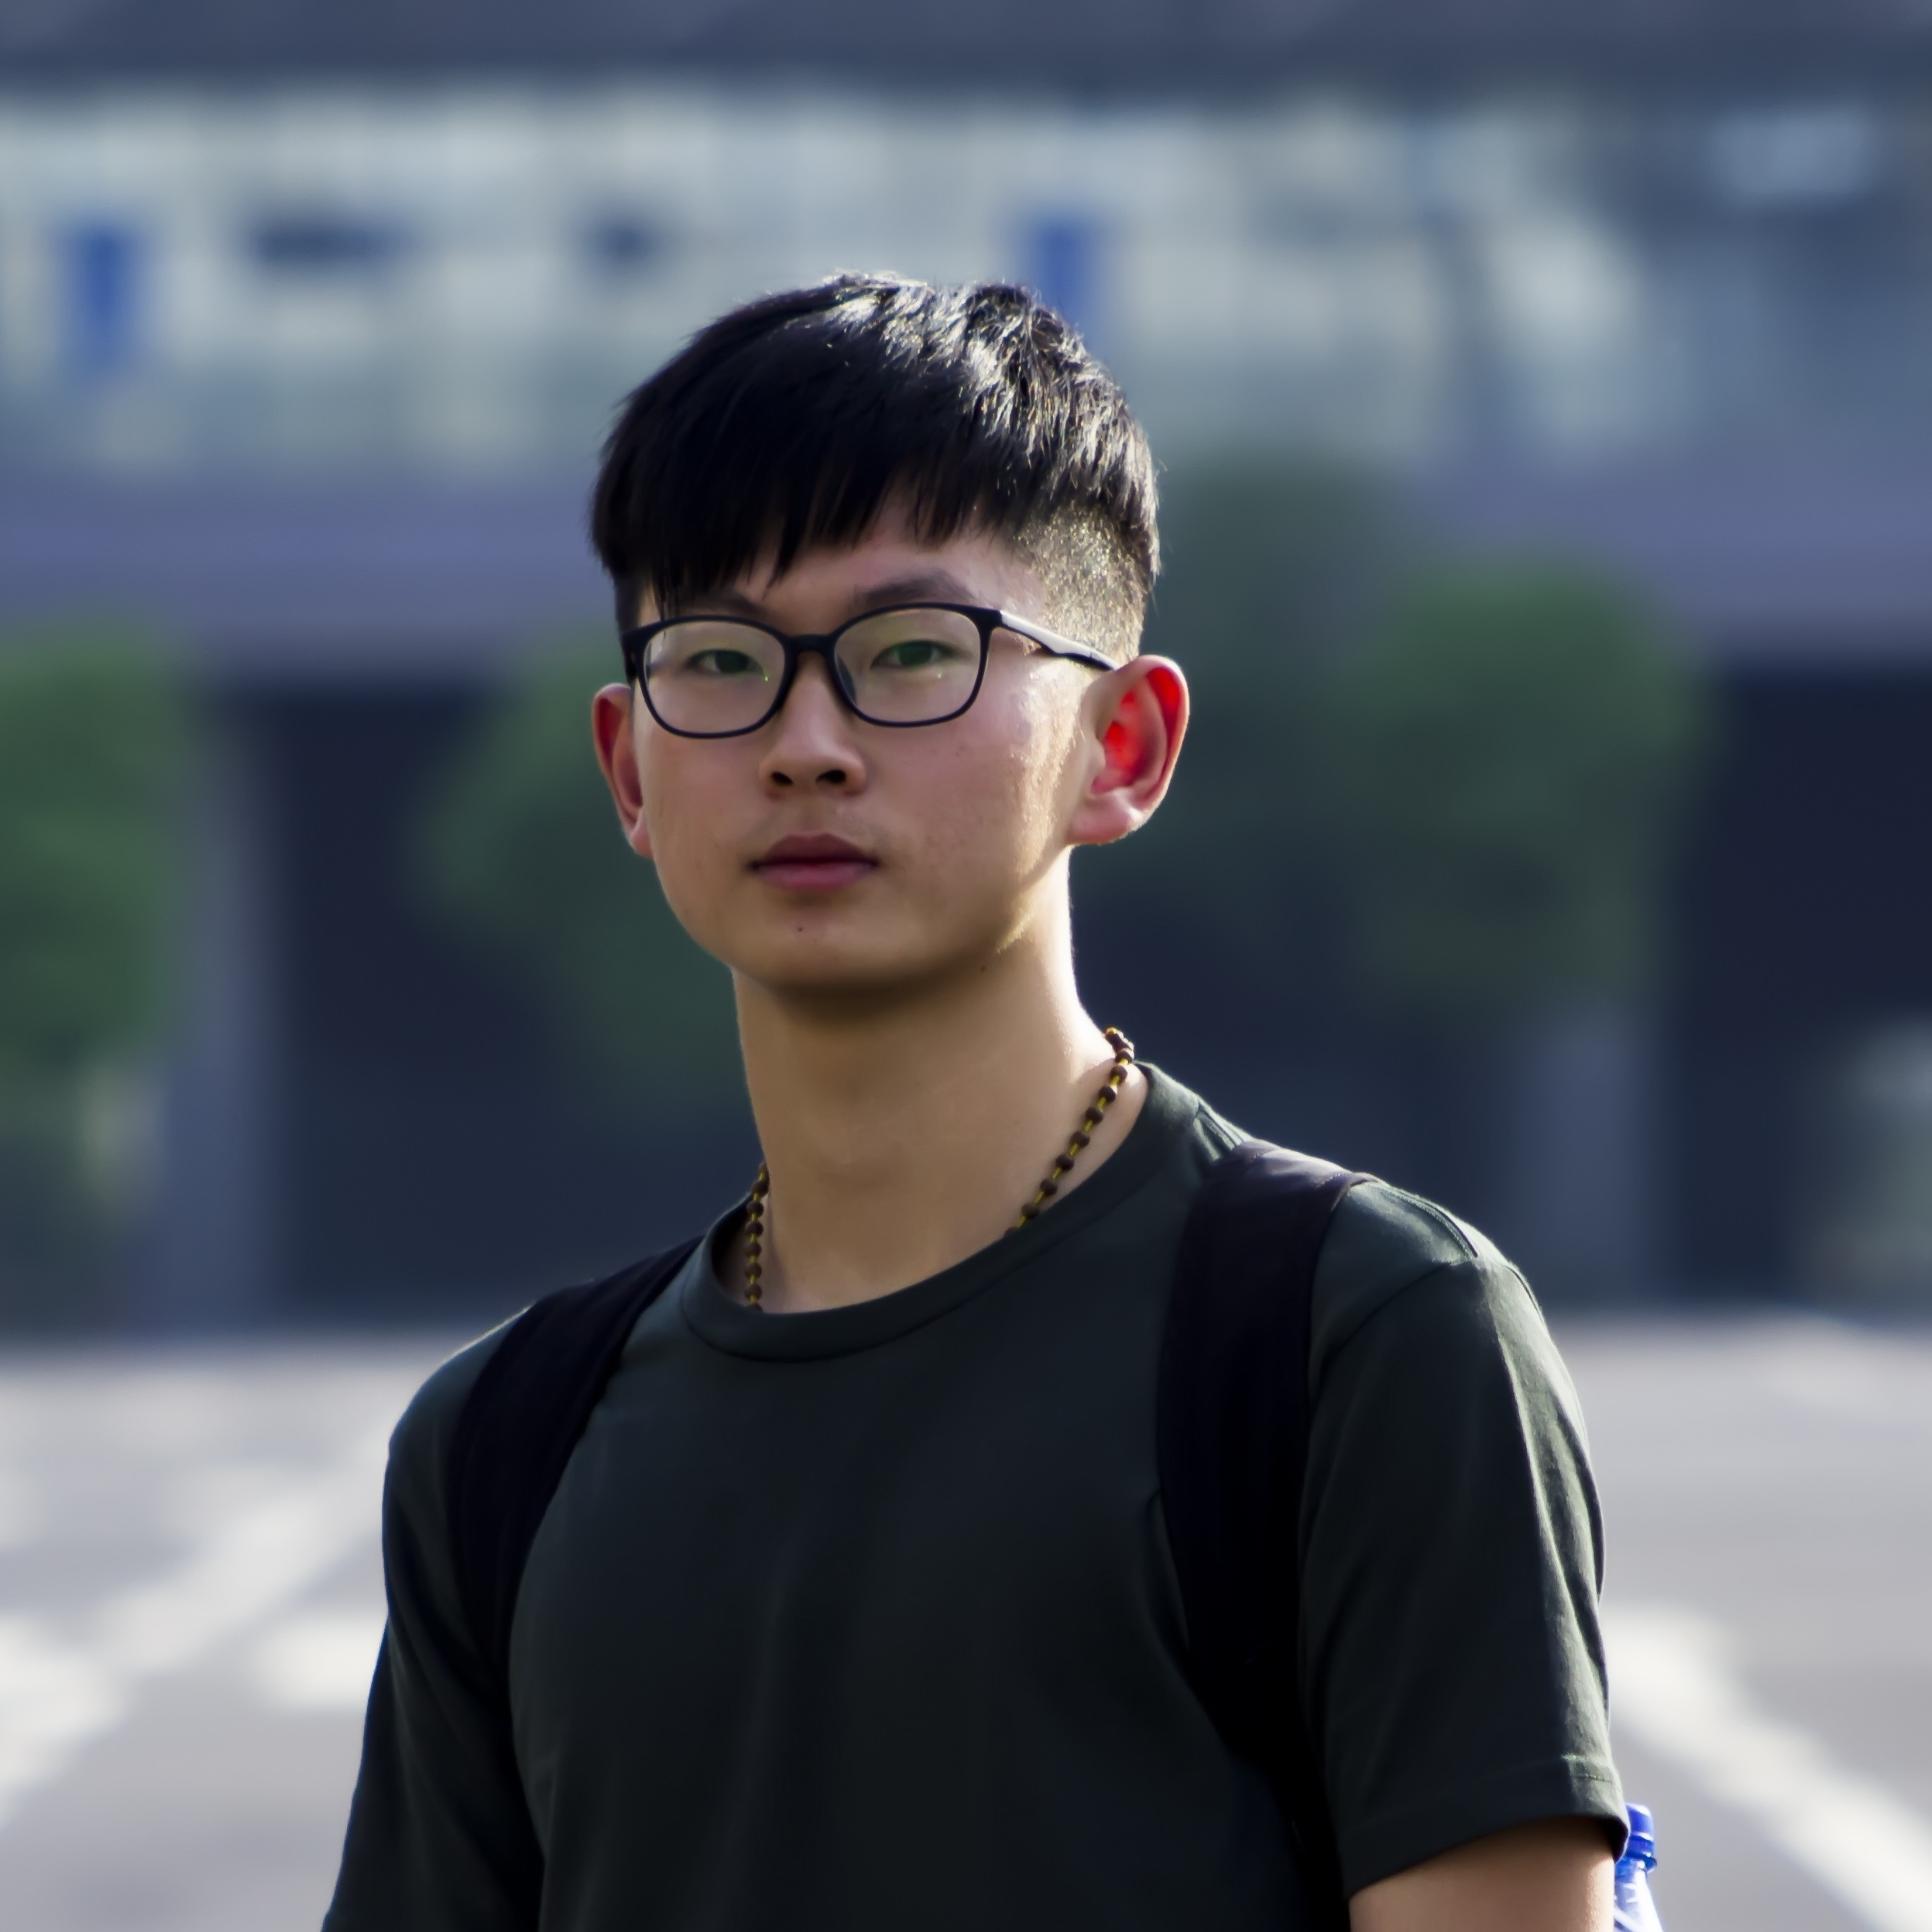
\includegraphics[width=3cm,height=0.7cm]{picture}}
%\cvitem {}{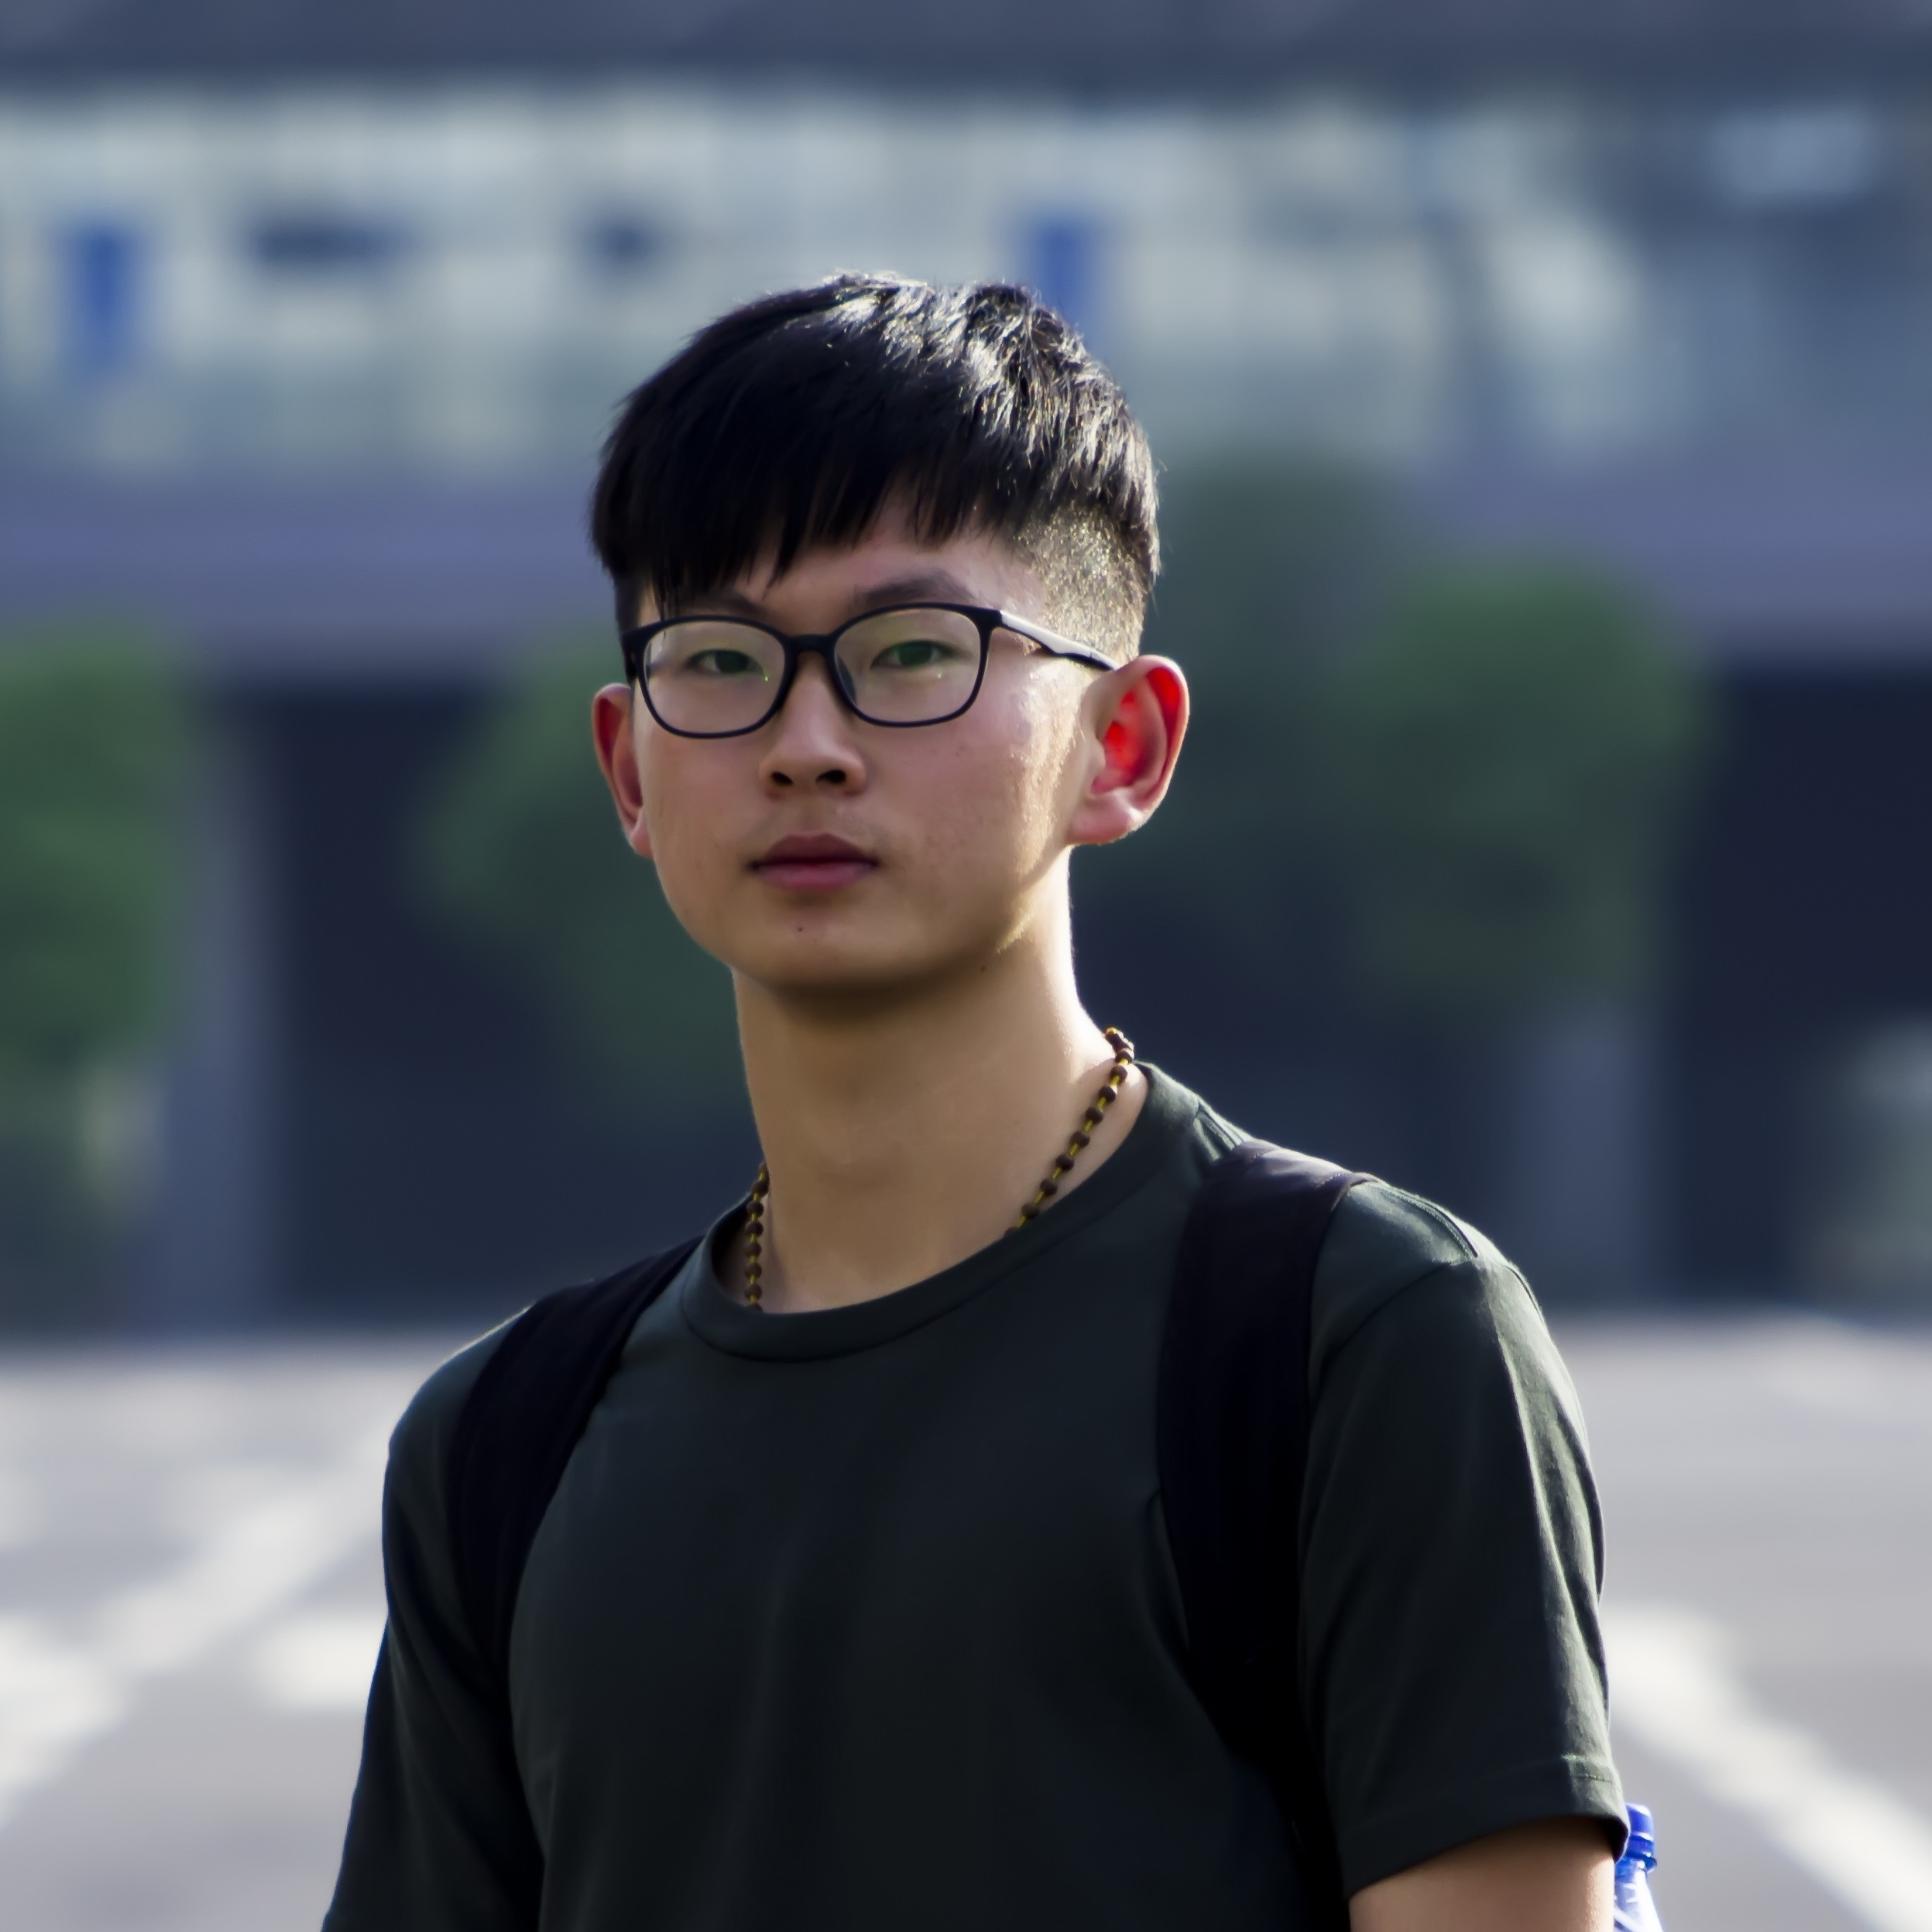
\includegraphics[width=3cm,height=0.7cm]{picture}}
%\cvitem {}{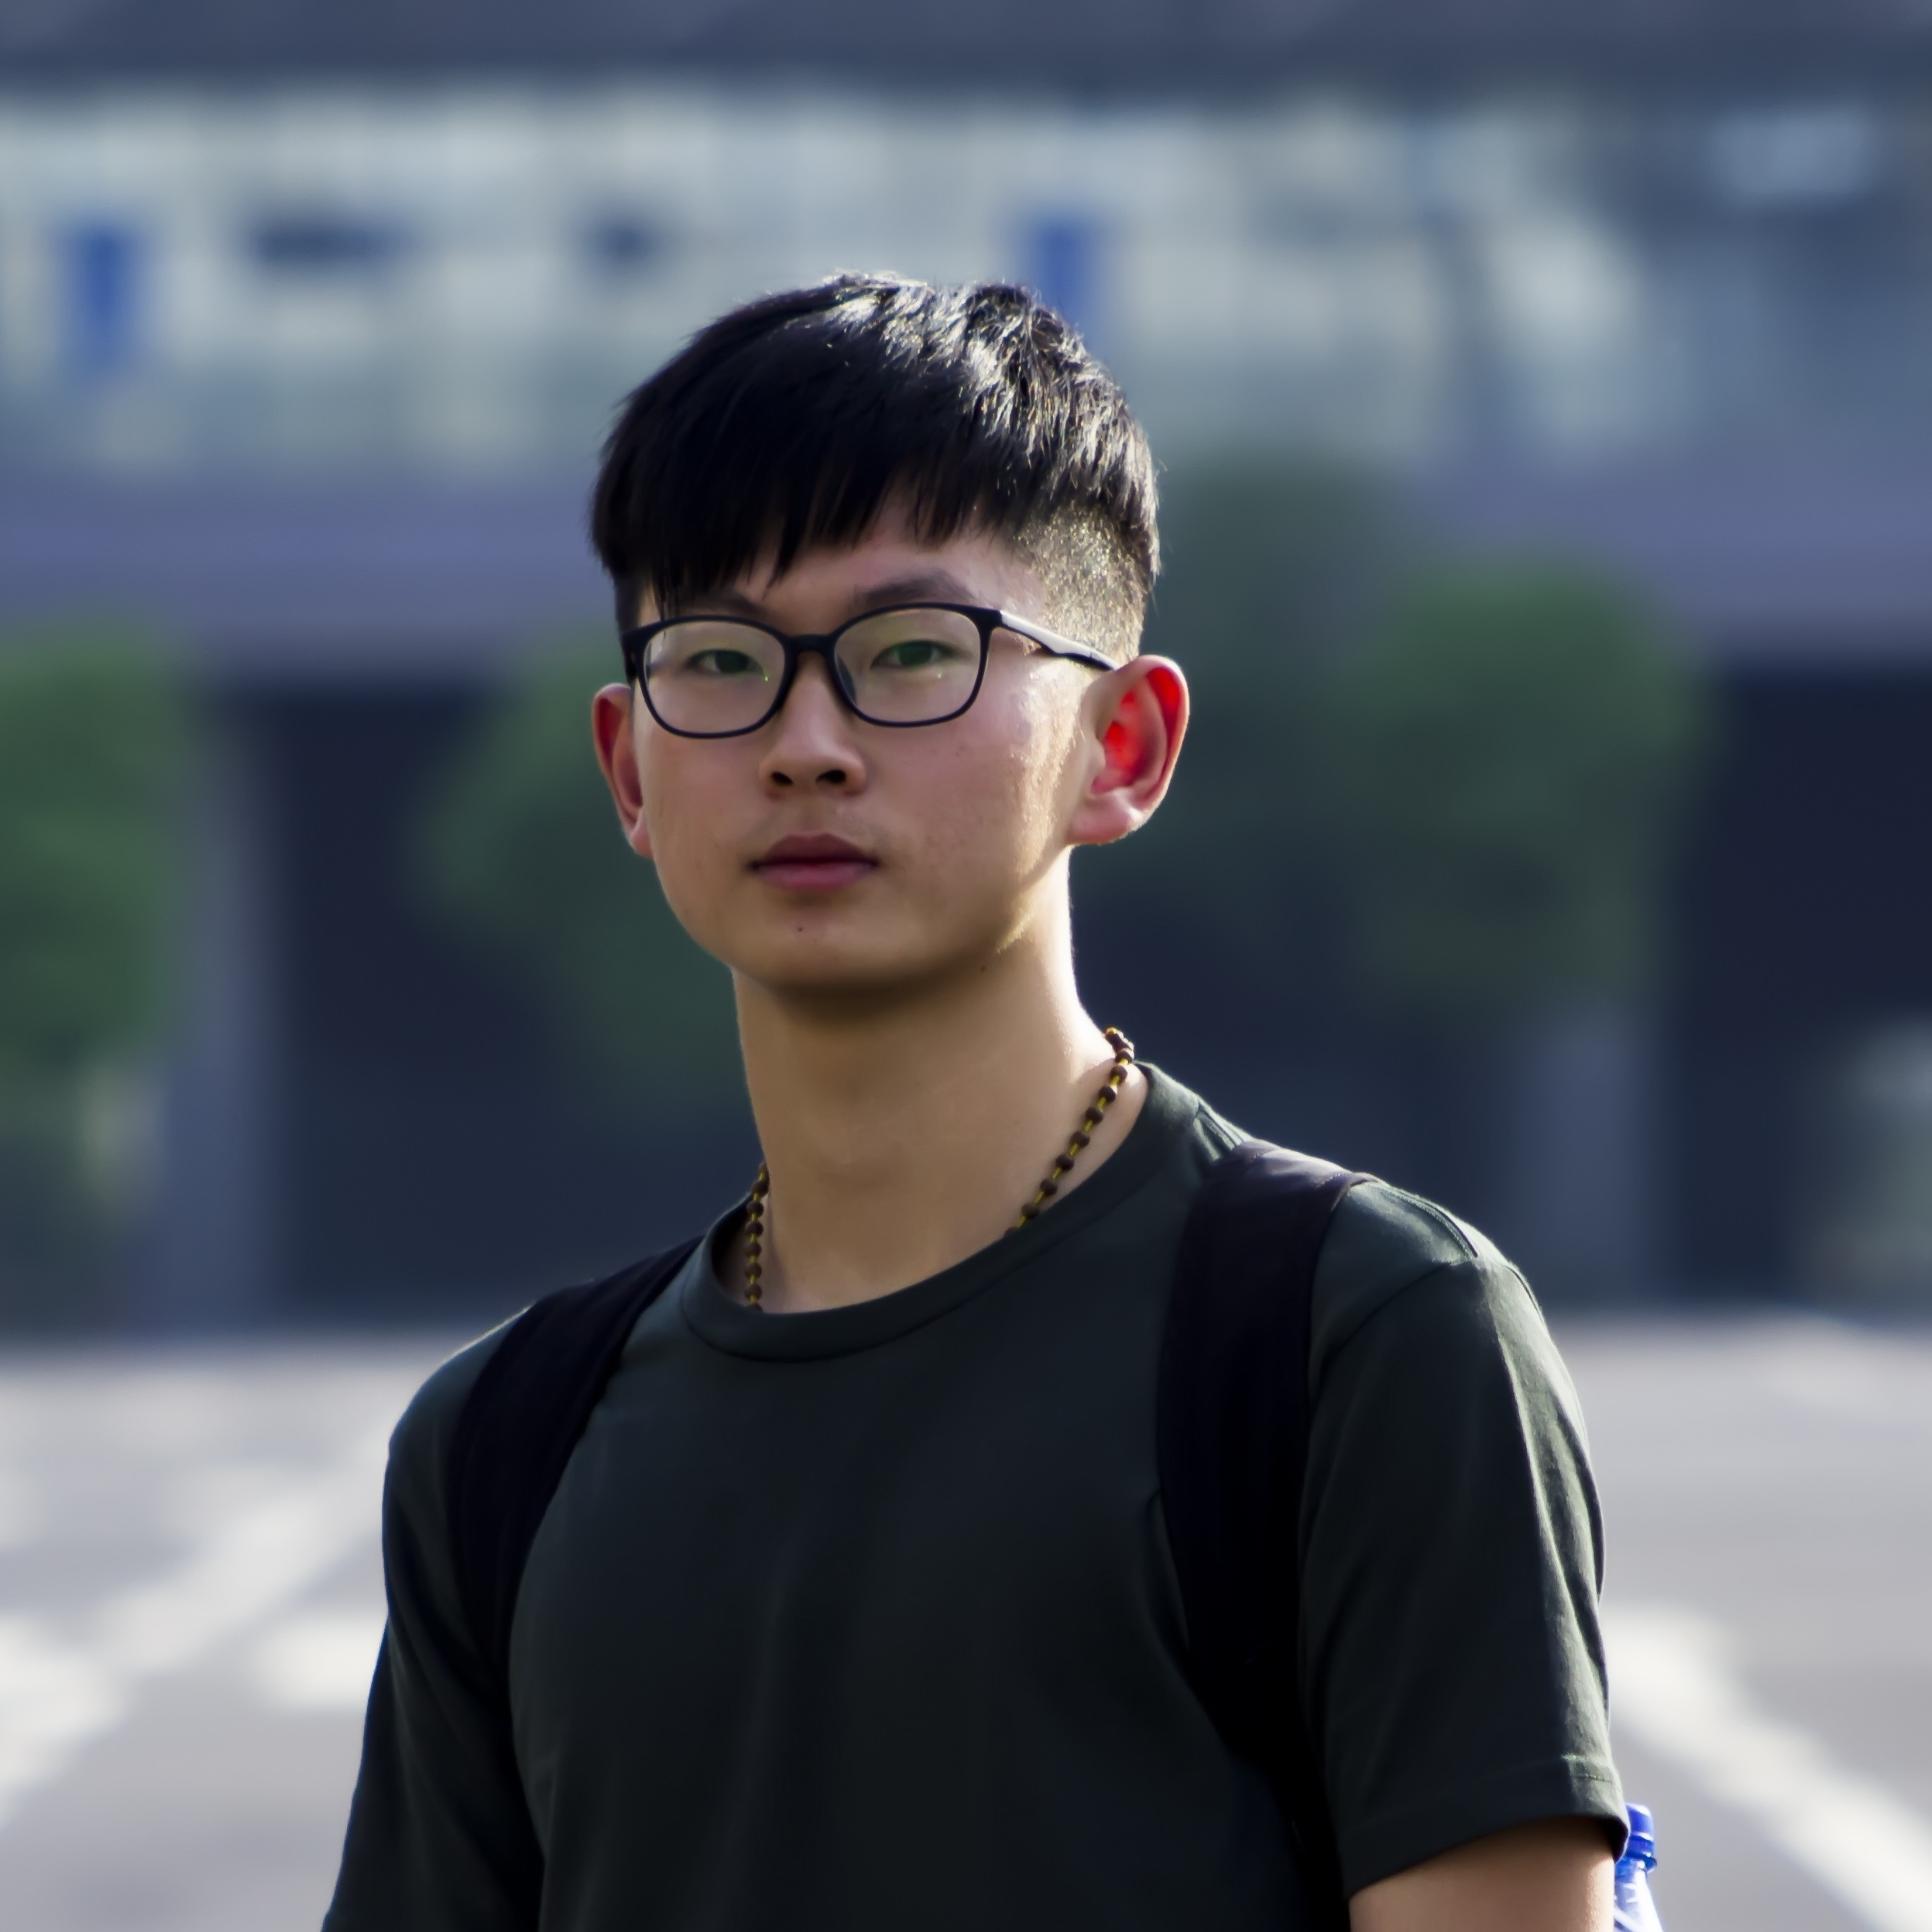
\includegraphics[width=3cm,height=0.7cm]{picture}}
%\end{multicols}
%\begin{multicols}{3}
%\cvitem {}{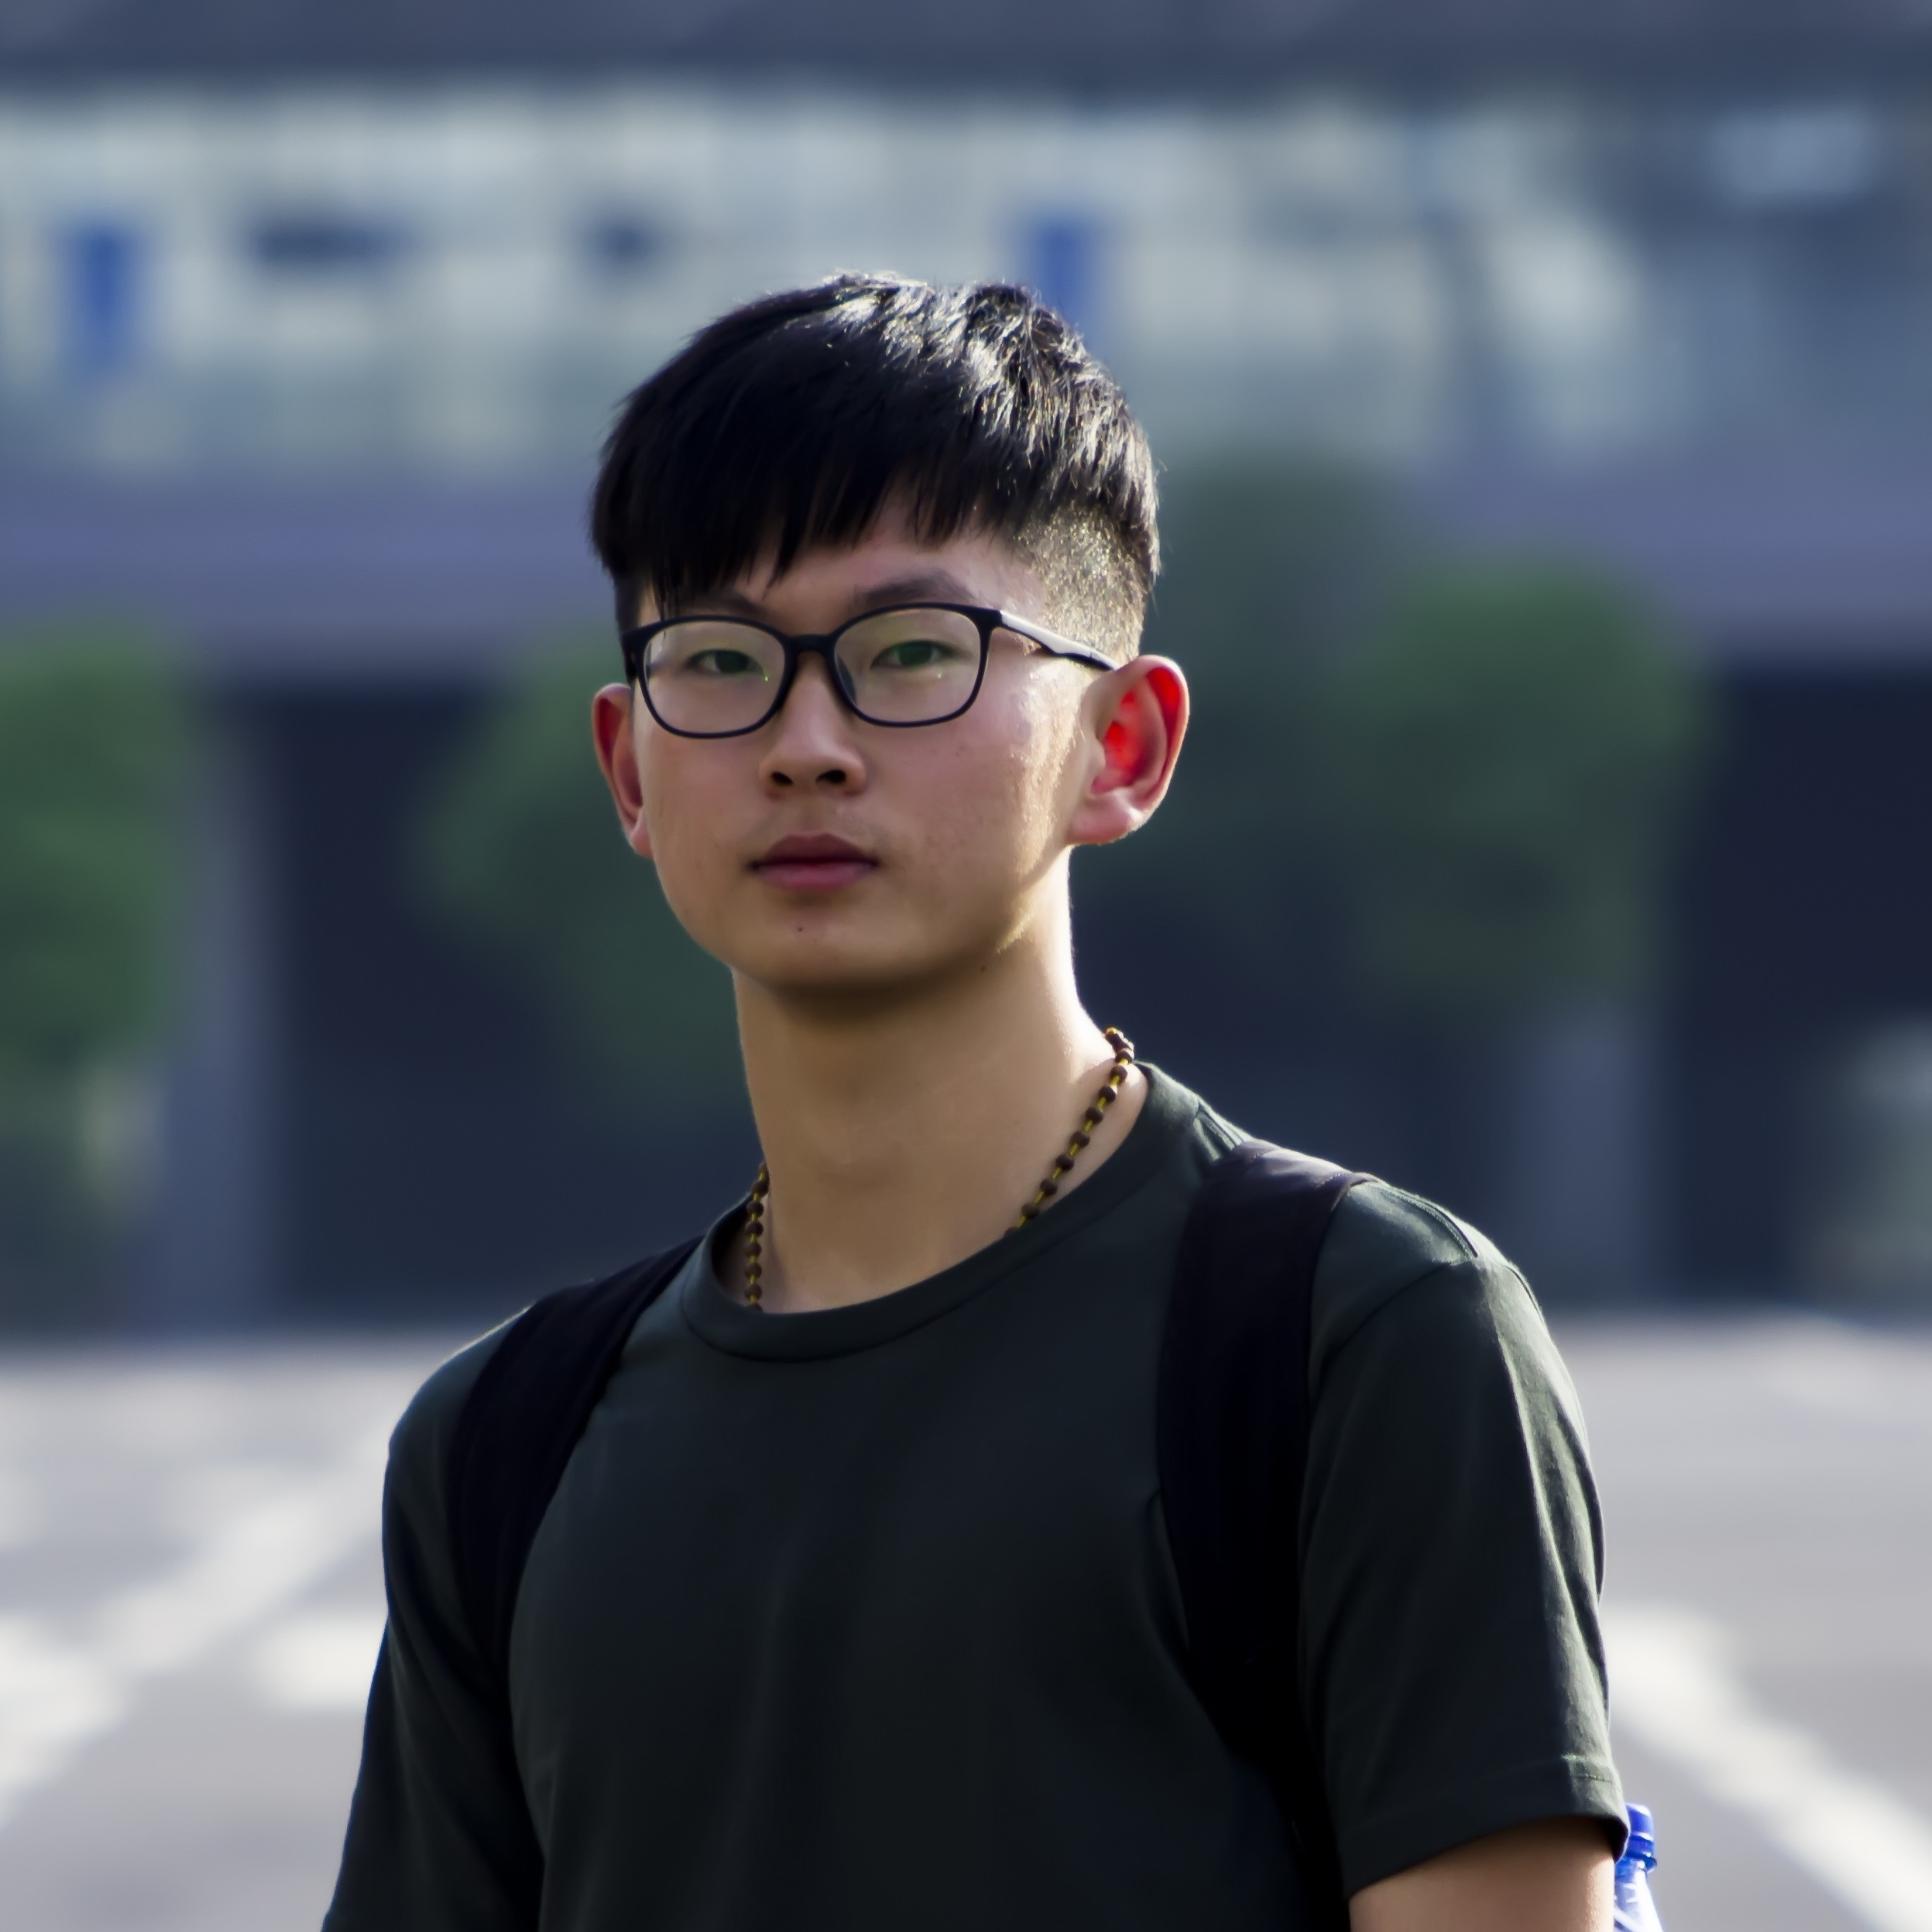
\includegraphics[width=3cm,height=0.7cm]{picture}}
%\cvitem {}{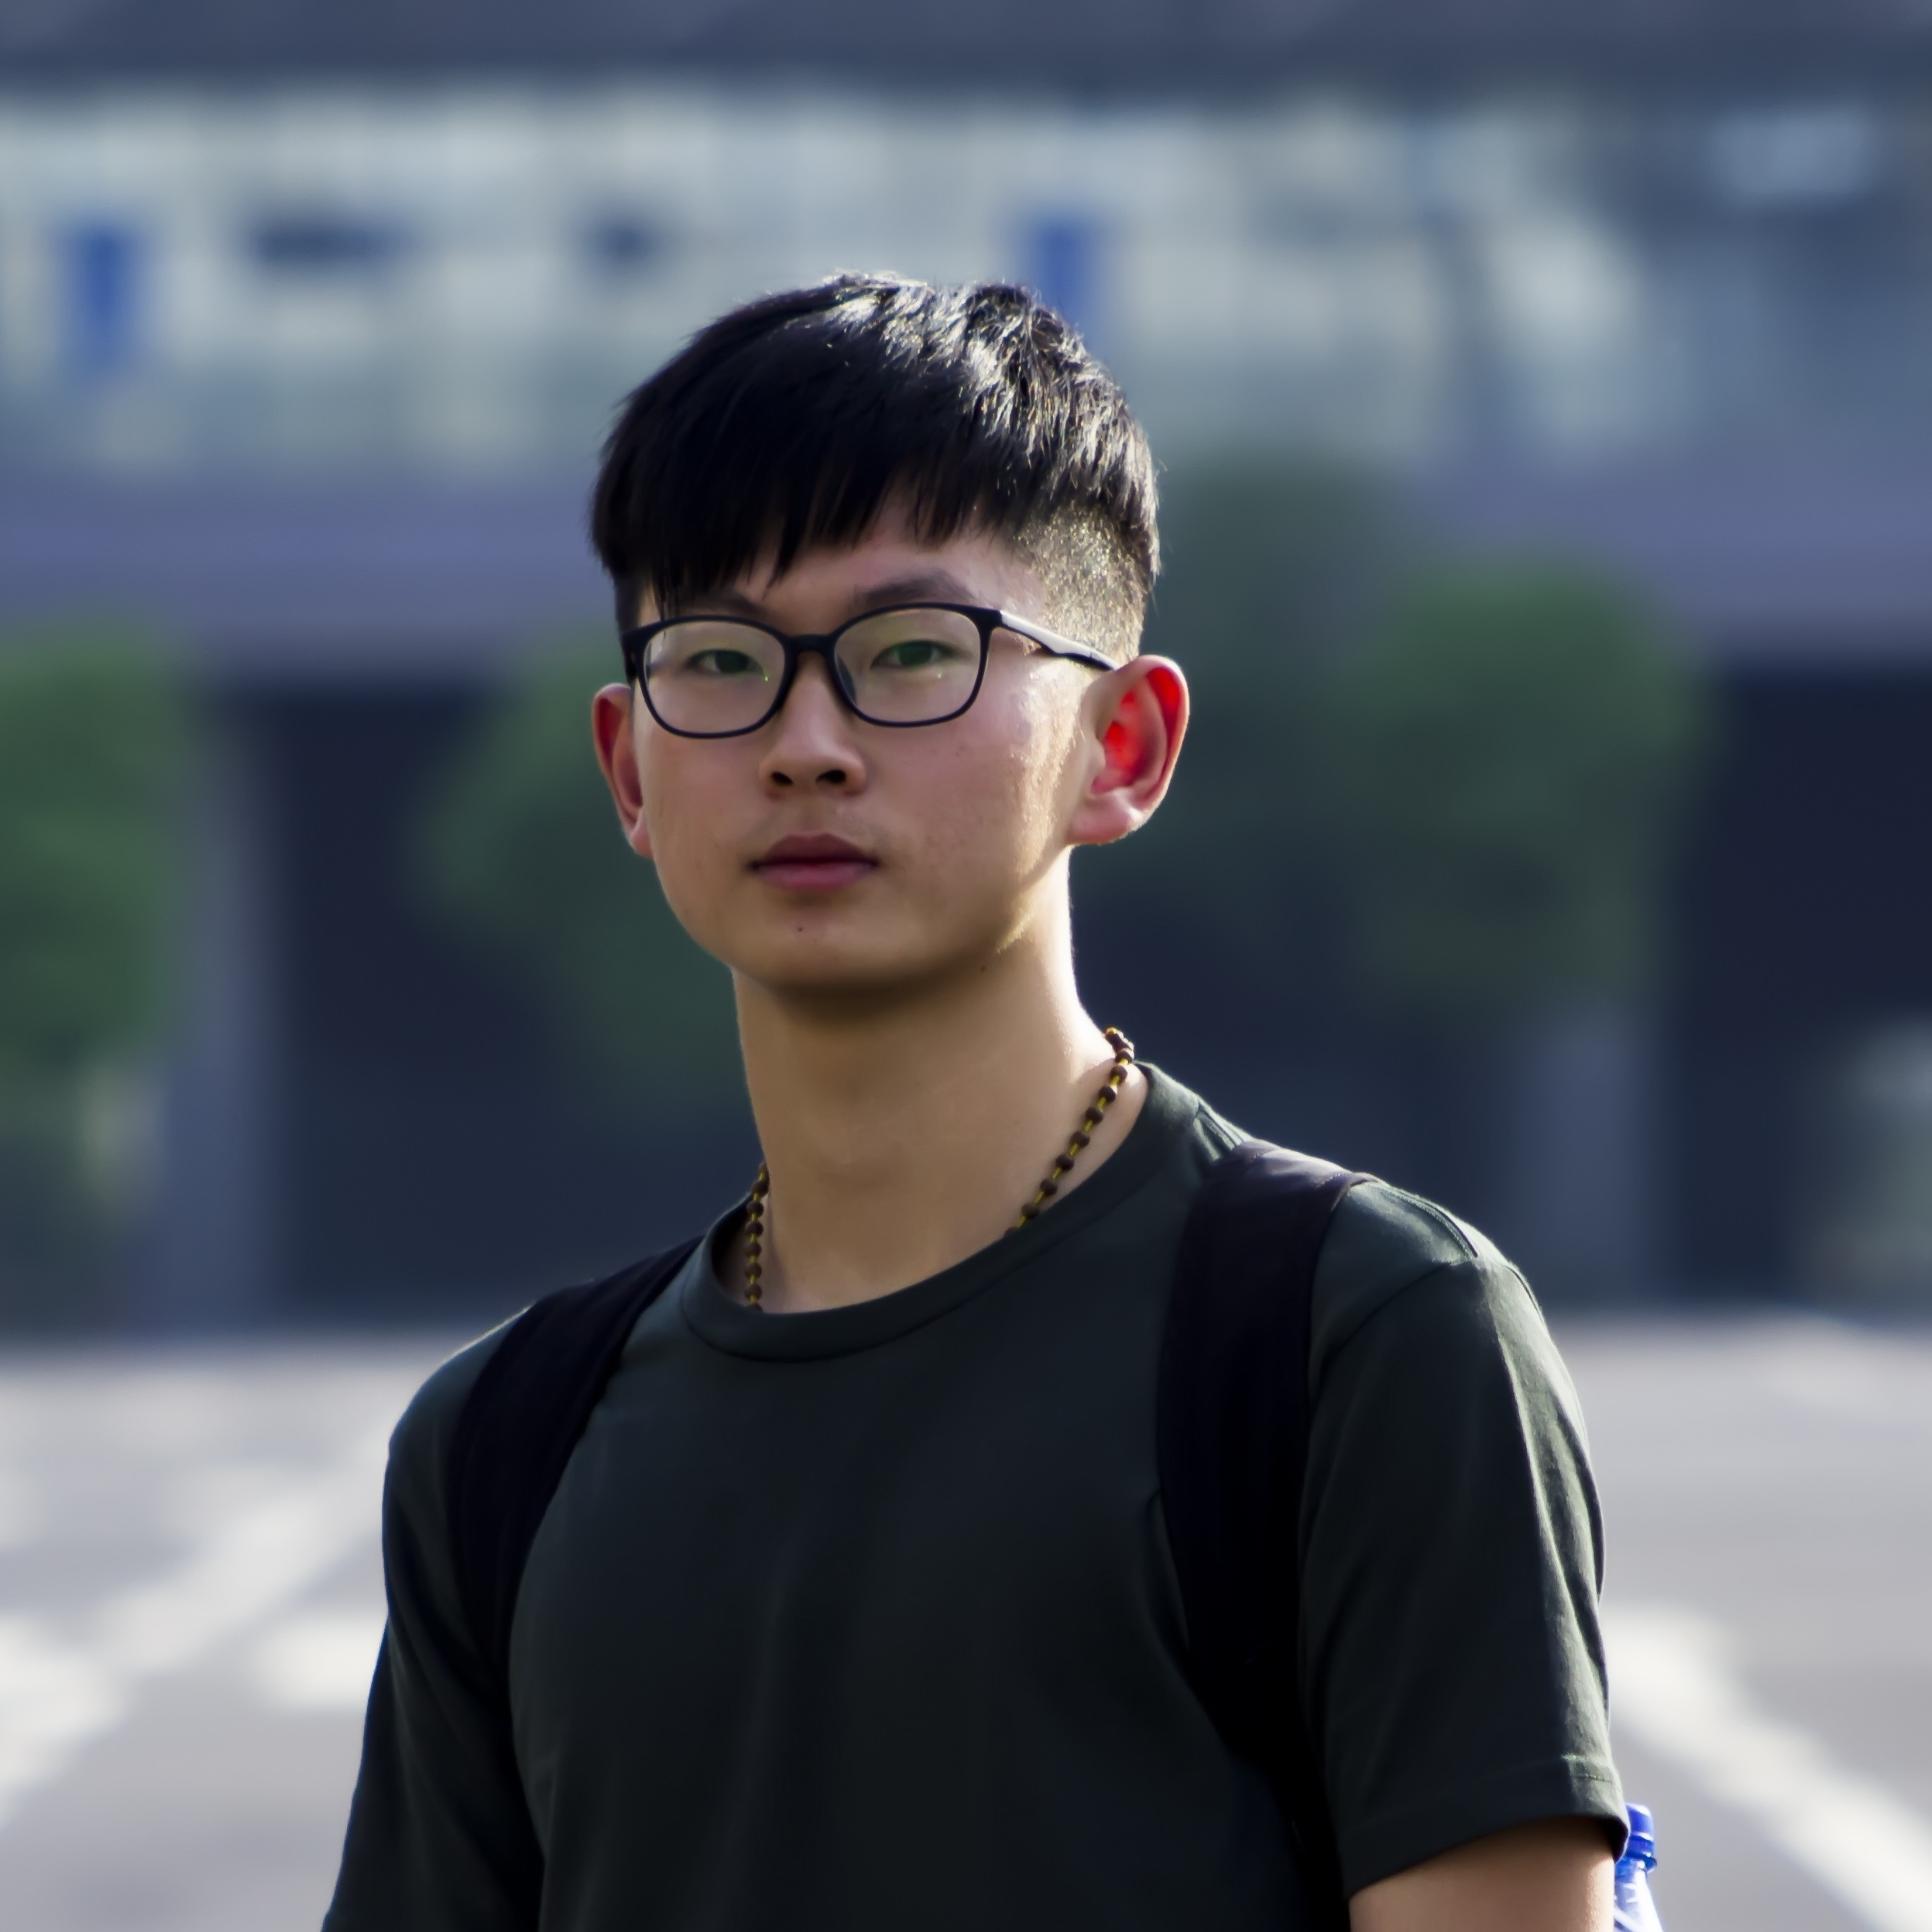
\includegraphics[width=3cm,height=0.7cm]{picture}}
%\cvitem {}{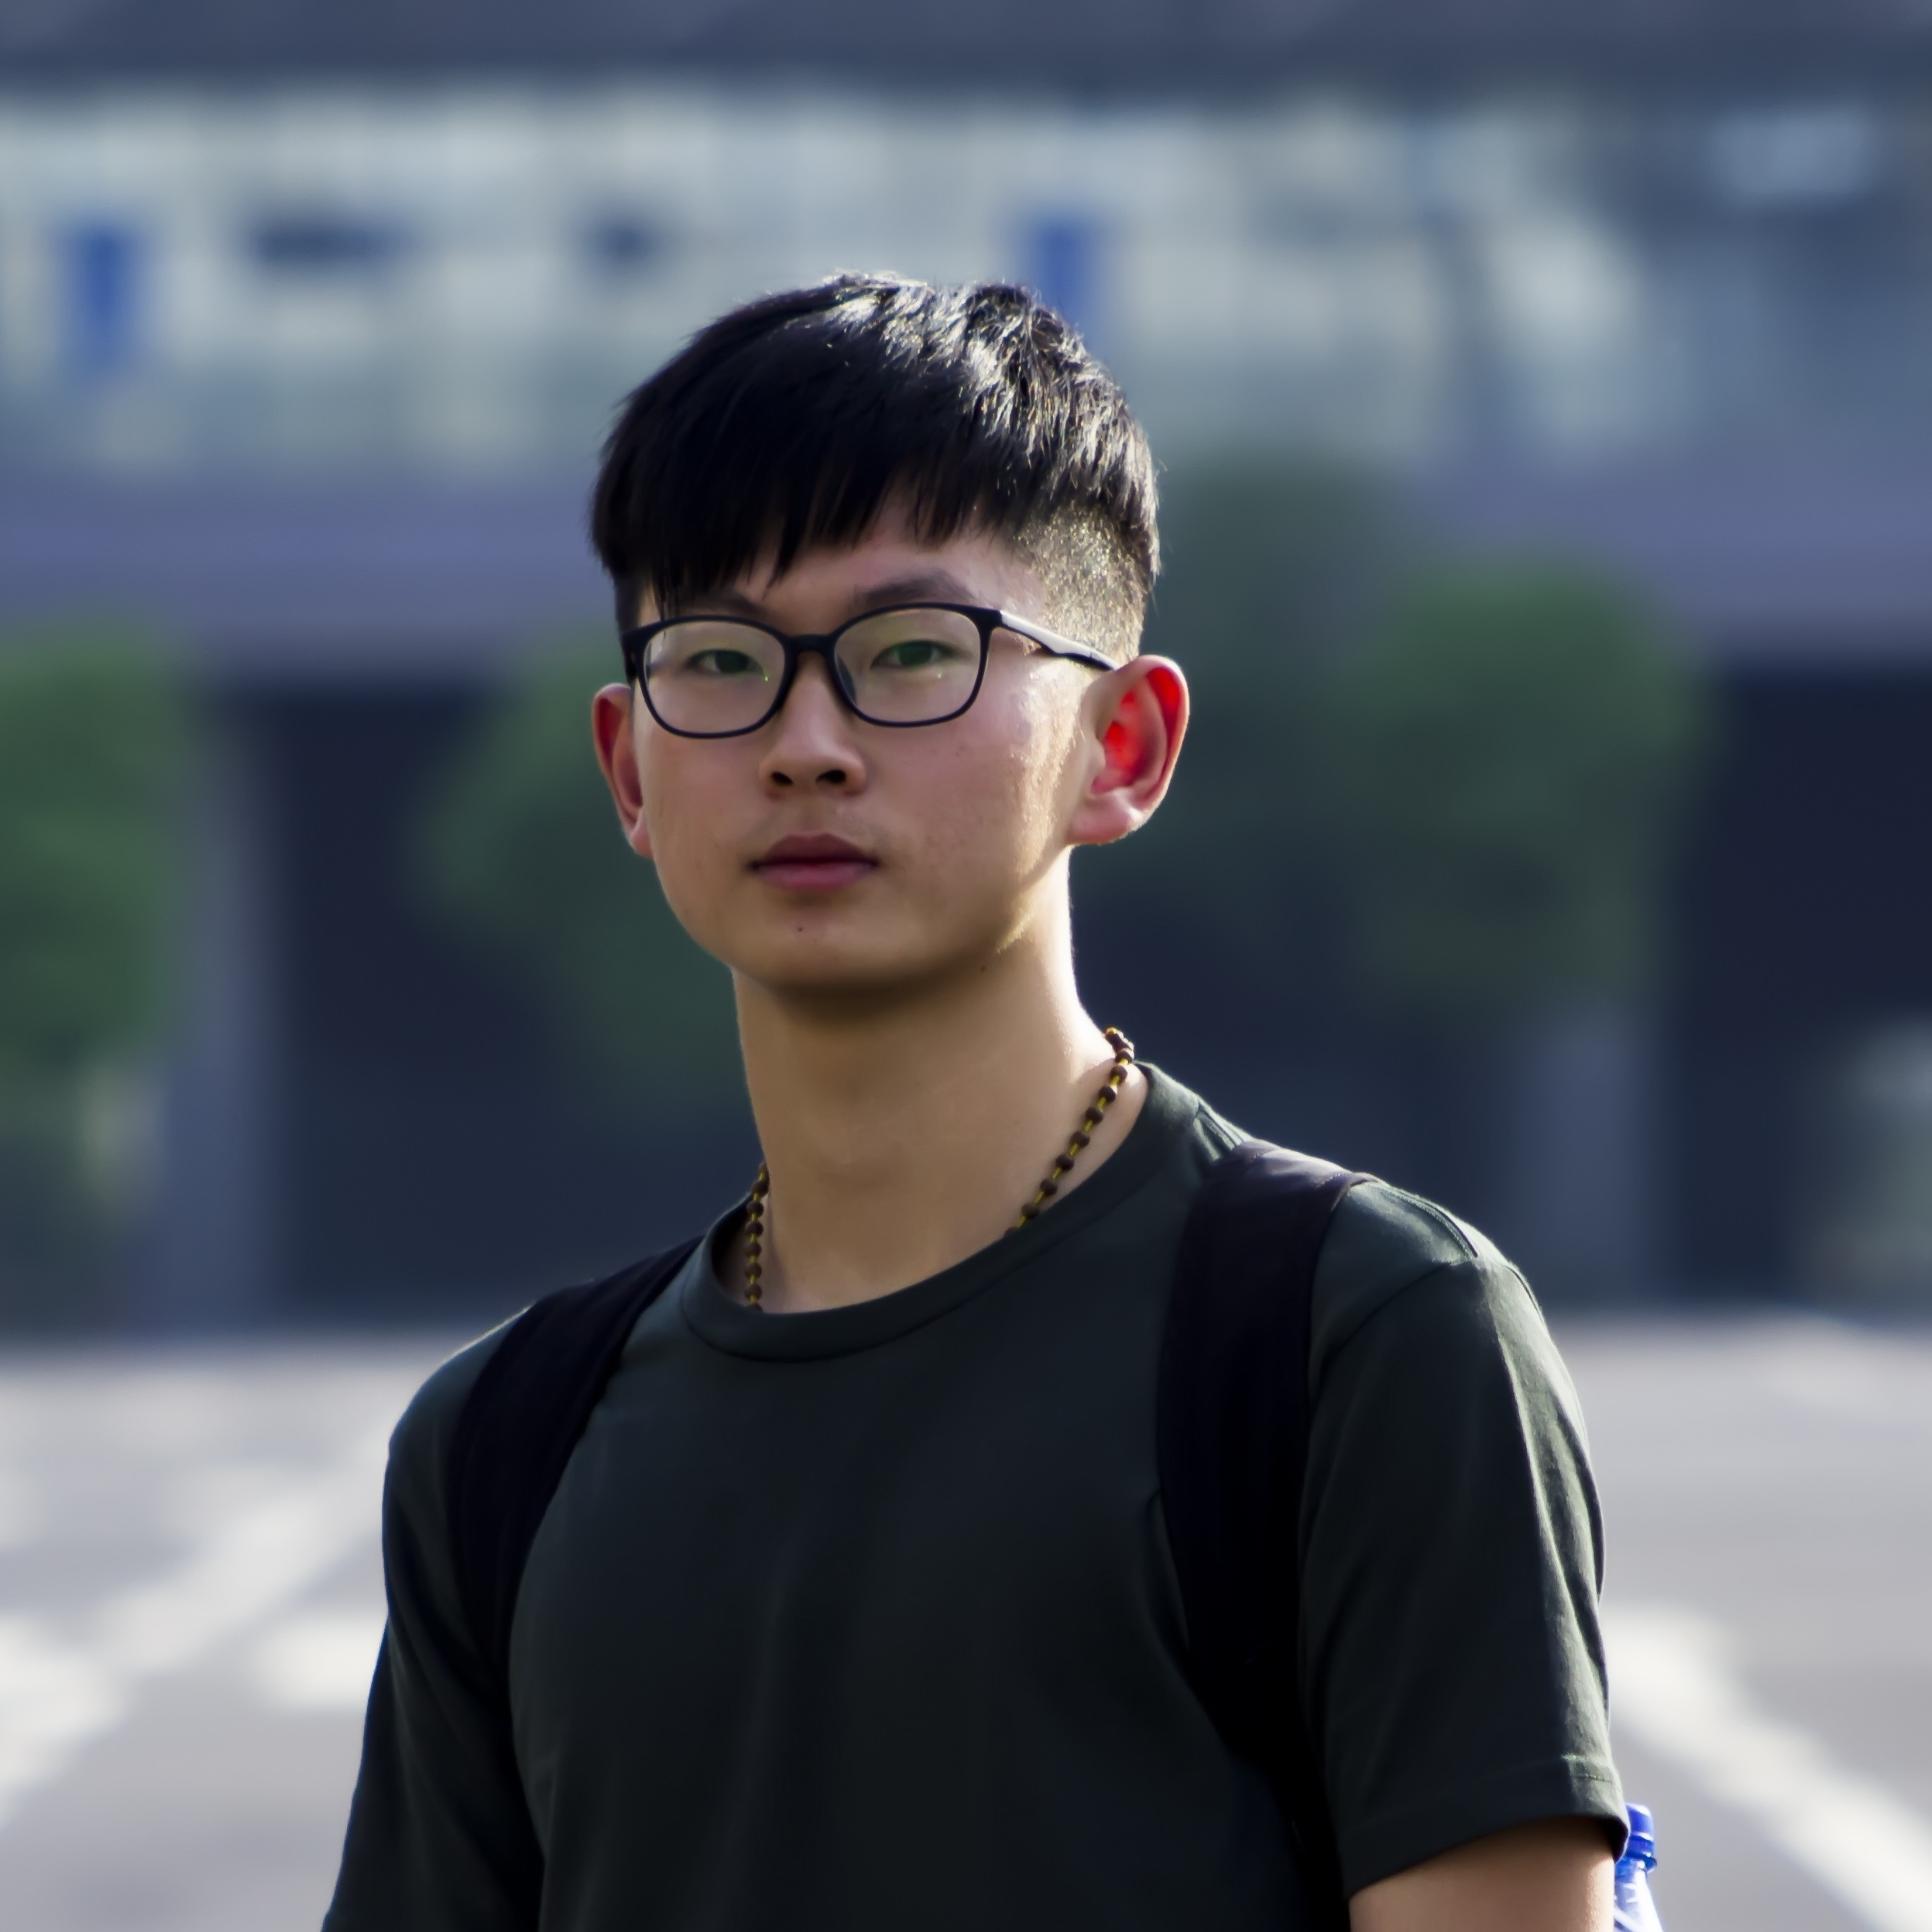
\includegraphics[width=3cm,height=0.7cm]{picture}}
%\end{multicols}
%\begin{multicols}{3}
%\cvitem {}{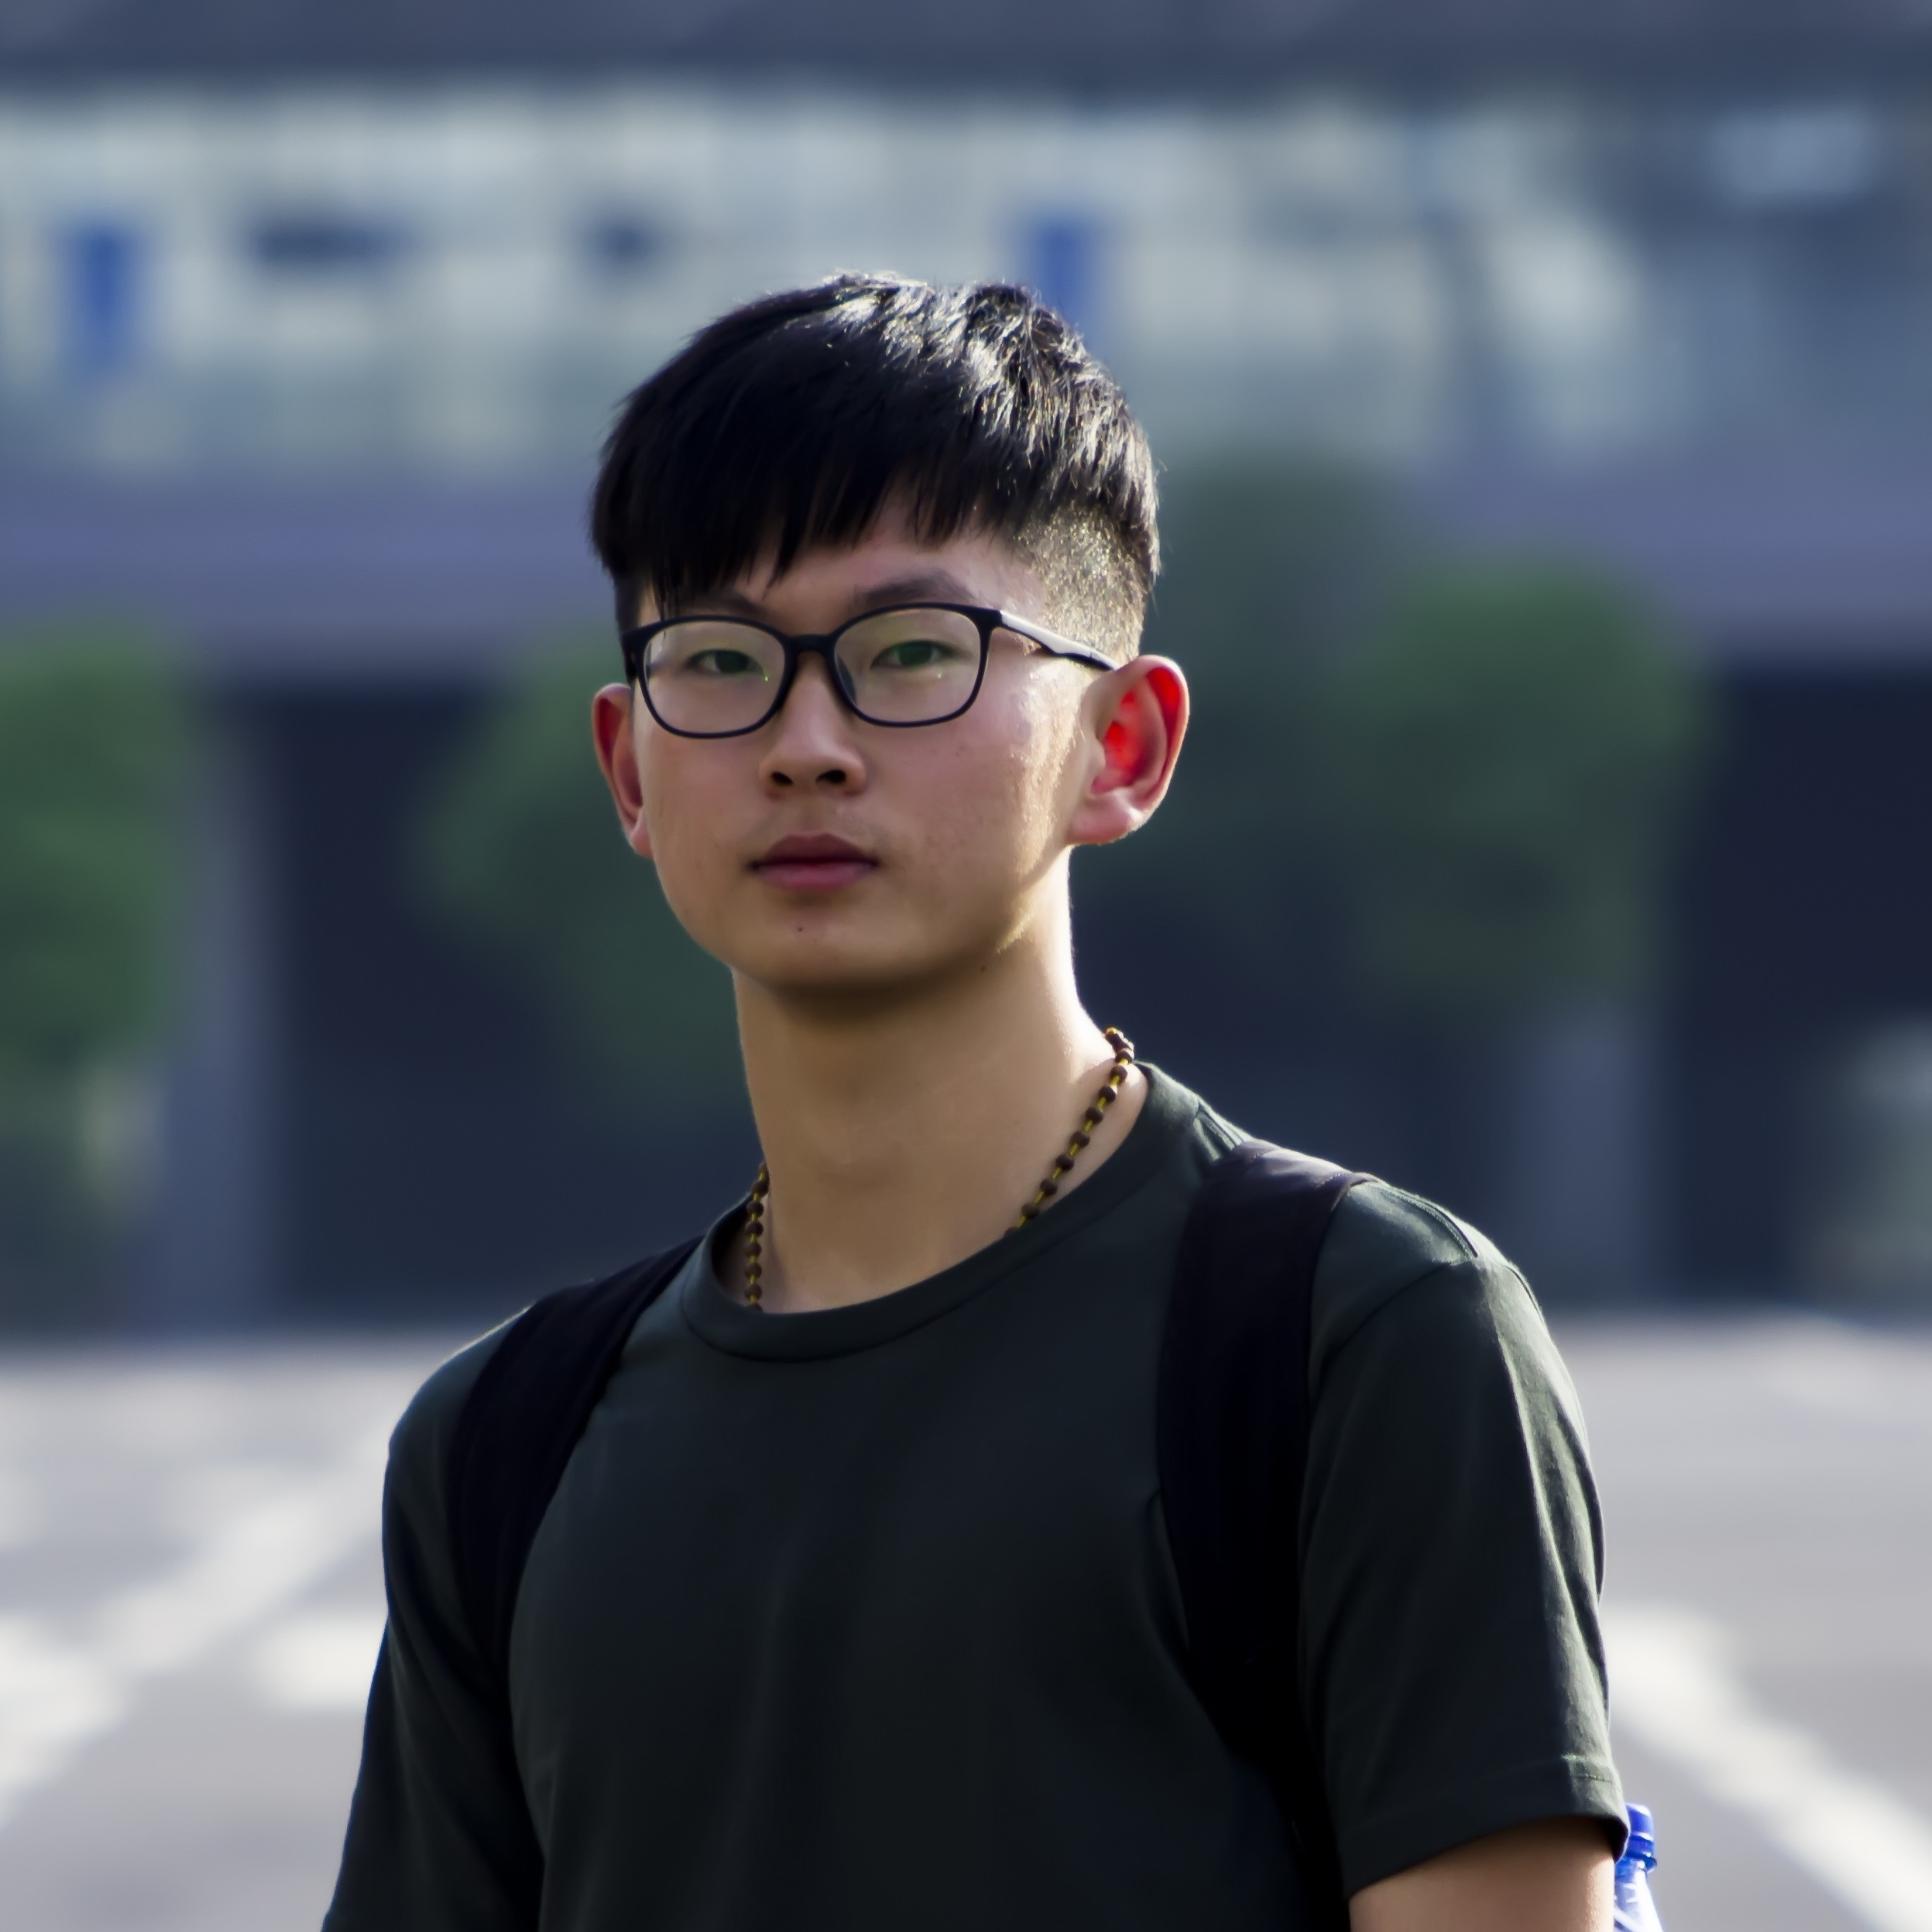
\includegraphics[width=3cm,height=0.7cm]{picture}}
%\cvitem {}{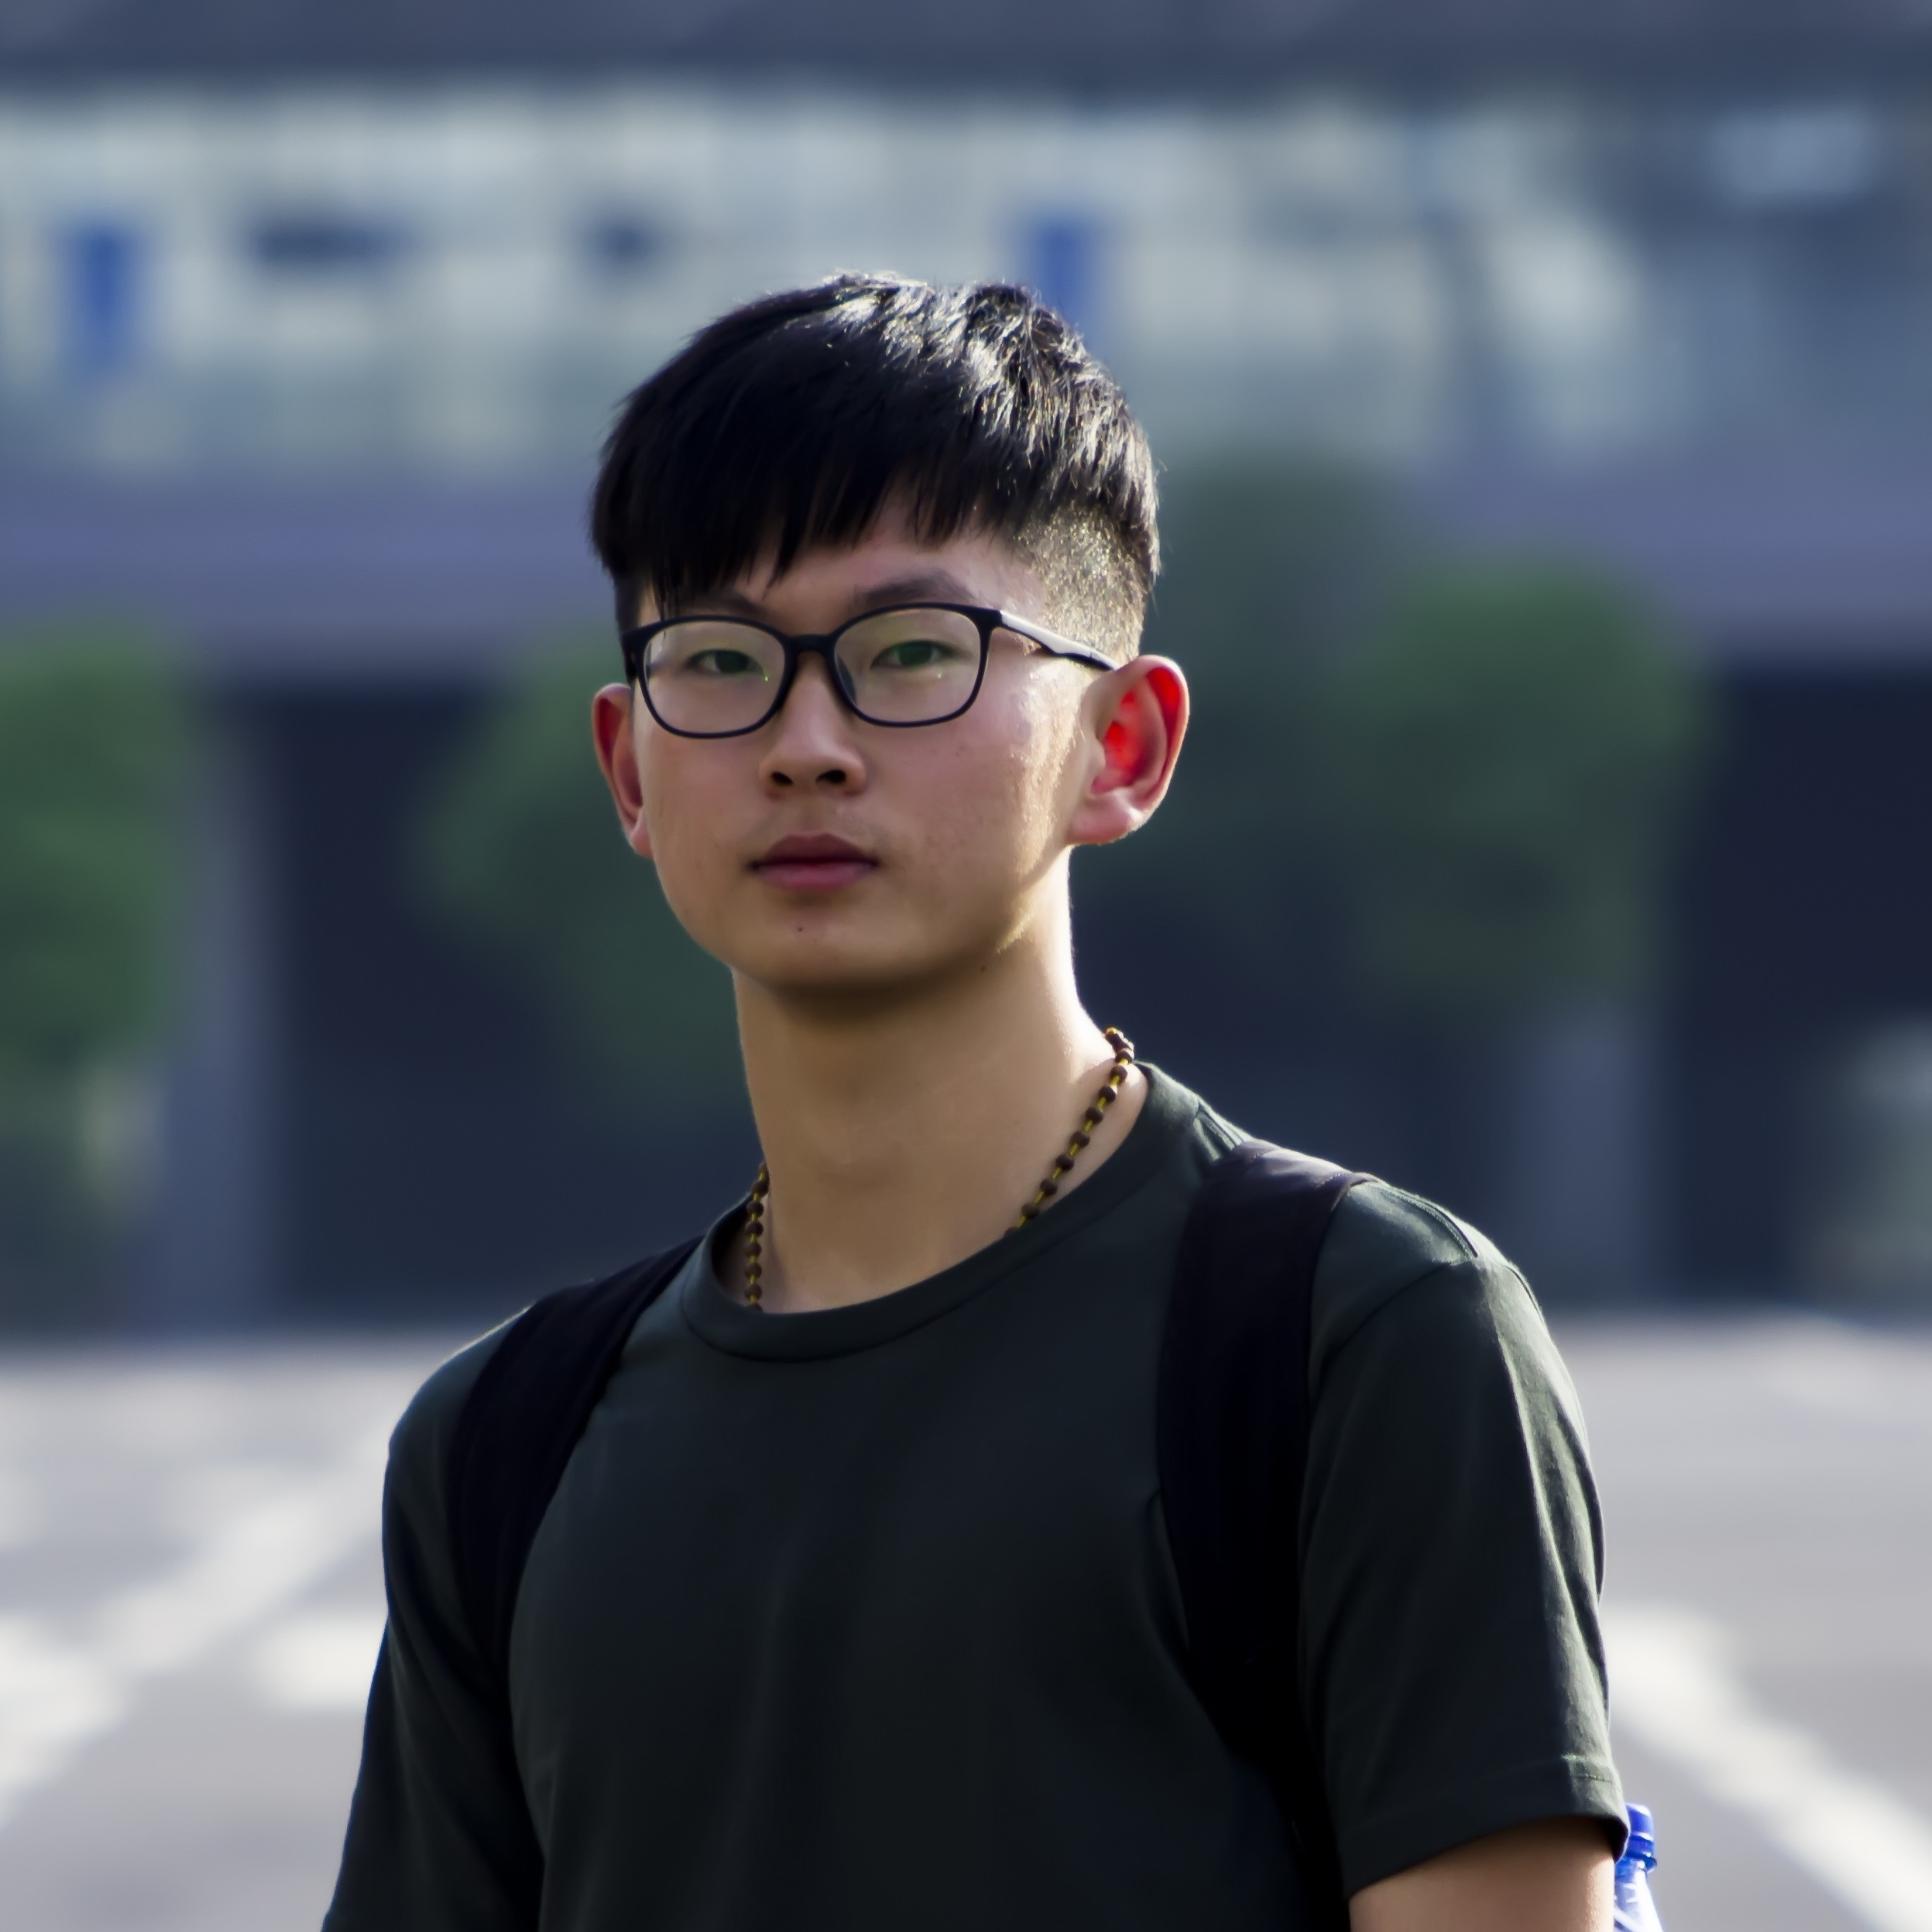
\includegraphics[width=3cm,height=0.7cm]{picture}}
%\cvitem {}{\includegraphics[width=3cm,height=0.7cm]%{picture}}
%\end{multicols}
%\subsection{Additional Softwares}
\begin{multicols}{3}
\cvitem{}{Microsoft Office}
\cvitem{}{Adobe Lightroom }
\cvitem{}{Adobe Photoshop}
\end{multicols}
\begin{multicols}{3}
\cvitem{}{C语言}
\cvitem{}{Java}
\cvitem{}{Visual Studio}
\end{multicols}

%\begin{multicols}{3}
%\cvitem{}{C}
%\cvitem{}{$C^{++}$}
%\cvitem{}{PageMaker}
%\end{multicols}

\section{个人品质}
\cvlistitem{组织能力强}
\cvlistitem{自学能力强}
\cvlistitem{有创造性思维}

%\section{Area of Interest}
%\cvlistitem{Finite Element Analysis}
%\cvlistitem{Engineering Graphics}
%\cvlistitem{Strenth of Material}
%\cvlistitem{Machine Design}

\section{获奖情况}
\cventry{2015-2016}{在大学中担任班长一职}{}{}{}{}
\cventry{2015}{获校区软件开发比赛二等奖}{}{}{}{}
\cventry{2015}{获校区级暑期社会实践优秀团队}{}{}{}{}
\cventry{2016}{所在班级获“优秀团支部”荣誉}{}{}{}{}
\cventry{2016}{获第七届“蓝桥杯”编程比赛JAVA组省三等奖}{}{}{}{}


%\cvlistitem{Held Technical Head \& Creativity Head position in college event ELYSIUM 14.}
%\cvlistitem{Participation in college competition ELYSIUM 12 and winner of Catapult.}


%----------------------------------------------------------------------------------------
%	LANGUAGES SECTION
%----------------------------------------------------------------------------------------

\section{考试等级}

\cvitemwithcomment{}{CET-4}{502}
\cvitemwithcomment{}{江苏省计算机等级}{专业四级}
%\cvitemwithcomment{Hindi}{Intermediate}{Conversationally fluent}
%\cvitemwithcomment{English}{Intermediate}{Can understand good}

%----------------------------------------------------------------------------------------
%	INTERESTS SECTION
%----------------------------------------------------------------------------------------

%\section{Interests}

%\cvlistdoubleitem{Painting}{Short Story Writing}
%\cvlistdoubleitem{Cooking}{Internet Surfing.}
%\cvlistitem{Cricket}


%\section{Declaration}
%\cvitem{}{I hereby declare that the above mentioned information is correct up to my
%knowledge and I bear the responsibility for the correctness of the above mentioned
%particular.}
%\cvitem{}{Date:}
%\cvitem{}{Place:}
%\cvitemwithcomment{}{}{\huge \color {black!20} 感谢阅读!}

\end{document}